\documentclass[a4paper, 12pt, openright]{report}

\usepackage[italian]{babel}
\usepackage{float}
\usepackage{graphicx}
\usepackage[utf8]{inputenc}
\usepackage{verbatim}
\usepackage{listings}     % per indice immagini
\usepackage[ruled,vlined]{algorithm2e}
%\usepackage{caption}
%\usepackage{algorithm}   % Pacchetto per scrivere algoritmi
%\usepackage{algorithmic}   % Pacchetto per scrivere algoritmi
\usepackage{makecell}
\usepackage{cellspace}
\setlength\cellspacetoplimit{6pt} % Spazio sopra il testo
\setlength\cellspacebottomlimit{6pt} % Spazio sotto il testo

\usepackage[hidelinks]{hyperref}






\graphicspath{{./images/}}

\newcommand{\emptypage}{
  \clearpage
  \pagenumbering{gobble}
  \mbox{}
}

\begin{document}

\begin{titlepage}
    \begin{center}
        \large
        Anno accademico 2022/2023 \\
        CORSO DI PROGETTAZIONE ALGORITMI

        \vfill

        \Huge
        \textbf{WePlay}

        \LARGE
        Documentazione di progetto
    \end{center}

    \vfill

    \begin{flushleft}
        \large
        \textbf{Irene Bravo} matr.~1071820 \\
        \smallskip
        \textbf{Samuel Locatelli} matr.~1054674 \\
        \smallskip
        \textbf{Greta Marrone} matr.~1058513
    \end{flushleft}

\end{titlepage}

\emptypage
\tableofcontents
\listoffigures


\chapter{Iterazione 0}
\pagenumbering{arabic}
\section{Requisiti}

Si vuole realizzare un sistema software che offra un servizio di sharing musicale, unito
alle funzionalità tipiche di un social network. Alla registrazione, l'utente dovrà
inserire una lista di generi musicali preferiti. L'algoritmo proporrà quindi all'utente i
brani più popolari basati sulle sue preferenze e gli permetterà di esplorare le sue
affinità musicali. Gli attori in gioco sono i seguenti:
\begin{itemize}
      \item utenti che vogliono ascoltare musica, conoscere e condividere le proprie
            attività musicali con gli amici;
      \item artisti indipendenti e non per pubblicare e gestire la propria musica.
\end{itemize}

L'utente, per poter usufruire dei servizi forniti, deve registrarsi e creare un proprio
profilo personale. Una volta iscritto, verrà indirizzato alla homepage che mostra i brani
più popolari dei generi preferiti dall'utente, la possibilità di cercare un brano
specifico e la sezione di impostazioni personali e social. Quando viene selezionato il
brano da scaricare, vengono fornite tutte le informazioni relative (titolo, artista,
album, anno di uscita, genere di appartenenza, numero di ascolti, durata del brano, casa
discografica).

Il software offre anche la possibilità di mettere ``like'' ai brani e di creare playlist
personalizzate. Nella propria libreria saranno quindi presenti le playlist dell'utente e
la playlist dei brani preferiti. L'interfaccia social permette invece di aggiungere gli
amici e di chattare con essi.

La funzionalità principale offerta dal servizio è l'algoritmo ``Discover'', che consente
di trovare i brani più apprezzati dalle persone che ascoltano gli stessi generi musicali
dell'utente così da permettergli di scoprire sempre nuove canzoni.

L'artista, a differenza dell'utente ascoltatore, può caricare brani singoli e album
inserendo i dati relativi alla propria produzione artistica.

L'utente, per poter usufruire dei servizi forniti, deve registrarsi e creare un proprio
profilo personale. Una volta iscritto, verrà indirizzato alla homepage che mostra i brani
più popolari dei generi preferiti dall'utente, la possibilità di cercare un brano
specifico e la sezione di impostazioni personali e social. Quando viene selezionato il
brano da scaricare, vengono fornite tutte le informazioni relative (titolo, artista,
album, anno di uscita, genere di appartenenza, numero di ascolti, durata del brano, casa
discografica).

Il software offre anche la possibilità di mettere ``like'' ai brani e di creare playlist
personalizzate. Nella propria libreria saranno quindi presenti le playlist dell'utente e
la playlist dei brani preferiti. L'interfaccia social permette invece di aggiungere gli
amici e di chattare con essi.

La funzionalità principale offerta dal servizio è l'algoritmo ``Discover'', che consente
di trovare i brani più apprezzati dalle persone che ascoltano gli stessi generi musicali
dell'utente così da permettergli di scoprire sempre nuove canzoni.

L'artista, a differenza dell'utente ascoltatore, può caricare brani singoli e album
inserendo i dati relativi alla propria produzione artistica.


\vspace{1cm}
\section{Studio di fattibilità}
Procedendo con una valutazione dei costi e dei benefici della possibile realizzazione del
presente sistema, è possibile concludere che i costi principali sono relativi alla
funzionalità di Discover e brani consigliati. 

Per realizzare questa funzionalità è
necessaria l'implementazione di un algoritmo che vada a studiare i gusti e le preferenze
di ogni singolo utente e, dopo la preliminare fase di raccolta dati, proporrà all'utente
una serie di brani in linea con le sue preferenze. 

Per quanto riguarda invece la
fattibilità in termini di tecnologie e strumenti per la realizzazione del sistema 
il costo principale da considerare è quello relativo allo sviluppo del software e il servizio di hosting sia 
della piattaforma che del database. 


\newpage
\section{Casi d'uso}
Di seguito vengono riportati i casi d'uso raggruppati in base all'attore coinvolto. Come
anticipato gli attori in gioco sono i seguenti:
\begin{itemize}
      \item Utente ascoltatore;
      \item Artista;
\end{itemize}

\vspace{0.5cm}
\subsection{Casi d'uso utente}
\begin{itemize}
      \item \textbf{UC1: Sign up} 
            
      L'utente può registrarsi inserendo le sue informazioni personali.
      \item \textbf{UC2: Sign in}
      
      L'utente può accedere al proprio profilo personale inserendo nome utente e password.
      \item \textbf{UC3: Sign out} 
      
      L'utente può disconnettere il proprio profilo personale dal sistema.     
      \item \textbf{UC4: Cerca brano}
      
      L'utente può digitare nella barra di ricerca per cercare un brano dal titolo.
      \item \textbf{UC5: Cerca album}
      
      L'utente può digitare nella barra di ricerca per cercare un album dal titolo.
      \item \textbf{UC6: Cerca Artista}
      
      L'utente può digitare nella barra di ricerca per cercare un artista dal nome.
      \item \textbf{UC7: Scarica brano}
      
      L'utente può scaricare il brano.
      \item \textbf{UC8: Like al brano} 
      
      L'utente può esprimere il proprio interesse per un brano mettendo like.
      \item \textbf{UC9: Aggiungi brano a playlist}
      
      L'utente può aggiungere alla lista di brani della playlist un brano selezionato.
      \item \textbf{UC10: Cerca Utente} 
      
      L'utente può cercare un utente per nome dalla barra di ricerca apposita (cerca album/artista).
      \item \textbf{UC11: Aggiungi Utente} 
      
      L'utente può aggiungere alla propria lista amici un utente selezionato.
      \item \textbf{UC12: Visualizza informazioni profilo} 
      
      L'utente può consultare le proprie informazioni personali inserite in fase di registrazione.
      \item \textbf{UC13: Modifica profilo} 
      
      L'utente può modificare le proprie informazioni personali inserite in fase di registrazione.
      \item \textbf{UC14: Elimina profilo} 
      
      L'utente può eliminare il proprio profilo dal sistema.
      \item \textbf{UC15: Visualizza playlist} 
      
      L'utente può consultare tutte le proprie playlist.
      \item \textbf{UC16: Crea nuova playlist} 
      
      L'utente può creare una nuova playlist nella quale aggiungere brani.
      \item \textbf{UC17: Elimina playlist}
      
      L'utente può eliminare una delle proprie playlist.
      \item \textbf{UC18: Modifica playlist} 
      
      L'utente può modificare una delle proprie playlist, per esempio modificando il nome o rimuovendo brani.
      \item \textbf{UC19: ``Discover''} 
      L'utente può consultare brani scelti per lui dal sistema e amici suggeriti in base alle sue preferenze musicali.

\end{itemize}

\subsection{Casi d'uso artista}
\begin{itemize}
      \item \textbf{UC20: Crea pagina artista} 
      
      L'artista per poter pubblicare musica deve creare una pagina artista inserendo le proprie informazioni personali.
      \item  \textbf{UC21: Visualizza pagina artista} 
      
      L'artista può consultare la propria pagina artista, dove vengono visualizzati i propri brani/album pubblicati.
      \item  \textbf{UC22: Aggiungi brano} 
      
      L'artista può pubblicare un nuovo brano inserendo le informazioni relative.
      \item  \textbf{UC23: Aggiungi album} 
      
      L'artista può pubblicare un nuovo album contenente i brani scelti.
      \item  \textbf{UC24: Personalizza pagina artista} 
      
      L'artista può decidere quali brani e album mettere in evidenza nella propria pagina artista.
      \item  \textbf{UC25: Consulta anagrafica} 
      
      L'artista può consultare l'anagrafica relativa agli ascolti e ai like dei brani e album pubblicati.

\end{itemize}


\vspace{1cm}
\subsection{Dettaglio casi d'uso}
Di seguito verranno analizzati più nel dettaglio i casi d'uso sopra citati, 
identificandone descrizione, attore e passi principali.

Gli utenti avranno la possibilità di registrarsi al sito per poter fruire dei servizi di streaming di musica. 
Al momento della registrazione sarà necessario inserire alcune informazioni personali di base come nome, cognome, email. 
Inoltre si dovrà inserire un nome utente identificativo e una password, necessari per il login. Nel caso in cui l'utente 
sia già registrato sarà necessario inserire solo questi campi per accedere al sistema. 

Al termine dell'iscrizione è possibile navigare nella Home page, la quale si suddivide in varie sezioni; ad esempio, 
viene offerta una selezione dei brani più ascoltati e scaricati dagli utenti. 

Una volta scelto il brano, per ognuno di essi vengono visualizzate alcune informazioni come il titolo del brano, 
il nome dell'artista e l'etichetta discografica di riferimento.

Alternativamente, è possibile cercare un brano dalla barra di ricerca (tramite il titolo, nome dell'artista o nome 
dell'album) e scaricarlo.

È offerta la possibilità di mettere like al brano e creare playlist personalizzate con i propri brani preferiti: 
visualizzando la propria libreria, infatti, è possibile visualizzare i Brani Preferiti e le proprie playlist. 

Come anticipato il sistema offre anche funzionalità di un social network: infatti dalla barra di ricerca è possibile 
cercare per nome utente i propri amici e aggiungerli, in modo tale da poter condividere le proprie preferenze musicali. 

Una delle funzionalità principali offerte dal sistema è chiamata Discover e consiste nel poter usufruire di playlist 
create ad hoc dal sistema per l'utente, tramite lo studio delle sue preferenze. 

Gli artisti potranno gestire e pubblicare la propria musica tramite varie funzionalità offerte dal sistema. Al momento 
della registrazione bisogna seguire la procedura classica di sign-in, in seguito in una sezione apposita è offerta la 
possibilità di creare la pagina artista, all'interno della quale verrà inserito il nome che apparirà pubblicamente, 
insieme ad altre informazioni personali. 

Dopo aver creato il proprio profilo artista si potrà accedere alla propria pagina per pubblicare le proprie tracce, 
album, playlist, personalizzandola. Ogni volta che viene pubblicato un brano è possibile inserire eventuali nomi di 
collaboratori, artisti che hanno partecipato al brano e scrittori di testo e musica. Ogni artista può scegliere la 
data dalla quale rendere accessibile il brano o l'album.







\newpage
\subsection{Diagramma dei casi d'uso}

In figura \ref{fig-uml-use-cases} è stato riportato il diagramma dei casi d'uso, dove sono stati inseriti quelli
già precedentemente descritti mettendoli in correlazione con il corrispettivo attore.

\begin{figure}[H]
      \centering
      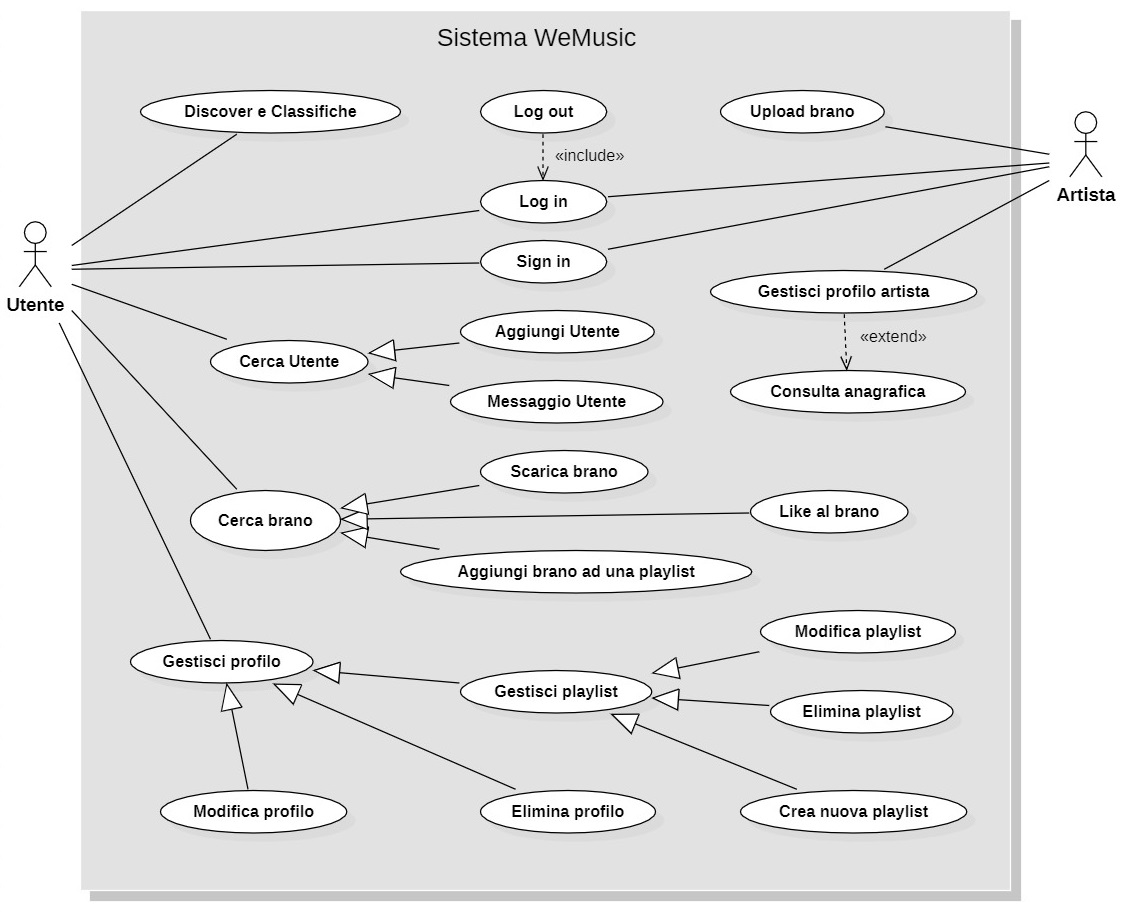
\includegraphics[scale=0.50]{UseCaseDiagram_ver2.jpg}
      \caption{UML Use Cases Diagram}
      \label{fig-uml-use-cases}
\end{figure}


\newpage
\section{Architettura del sistema}
L'architettura del sistema è stata formalizzata attraverso la rappresentazione tramite Deployment Diagram, diagramma di tipo statico 
sviluppato al fine di modellizzare e descrivere un sistema in termini di risorse hardware e di relazioni fra di esse.
Vengono sviluppatidue Deployment Diagram differenti:

il primo, riportato in figura \ref{architettura}, rappresenta il sistema
attraverso una notazione a stile libero, mentre il secondo, riportato in figura \ref{dep_diagram}, rappresenta
la topologia del sistema tramite lo stile UML. 

\vspace{2cm}

\subsection{Deployment diagram -- Informal}
In figura \ref{architettura} viene evidenziata la componente principale del sistema, il sistema gestore (WeMusic)
il Web Server (sviluppato tramite il framework Django) che, tramite una connessione ad internet, permette 
agli utenti di poter consultare il sito.
\begin{figure}[H]
      \centering
      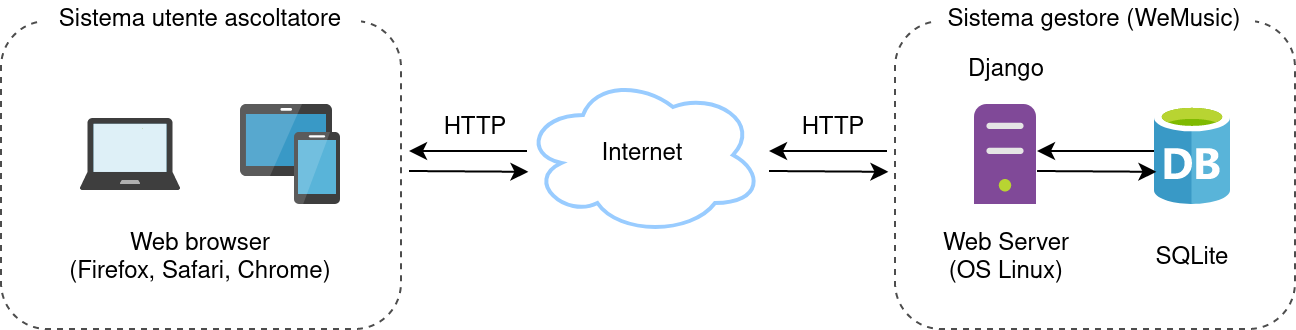
\includegraphics[width=\textwidth]{architettura.png}
      \caption{Architettura}
      \label{architettura}
\end{figure}


\newpage
\subsection{Deployment diagram -- UML}
In figura \ref{dep_diagram} vengono evidenziati due nodi principali: 
un lato client che gestirà il front-end del sistema WeMusic, e un lato server relativo 
al back-end e alla gestione del DataBase, in modo da velocizzare e semplificare l'interazione tra logica e dati. 
\begin{figure}[H]
    \centering
    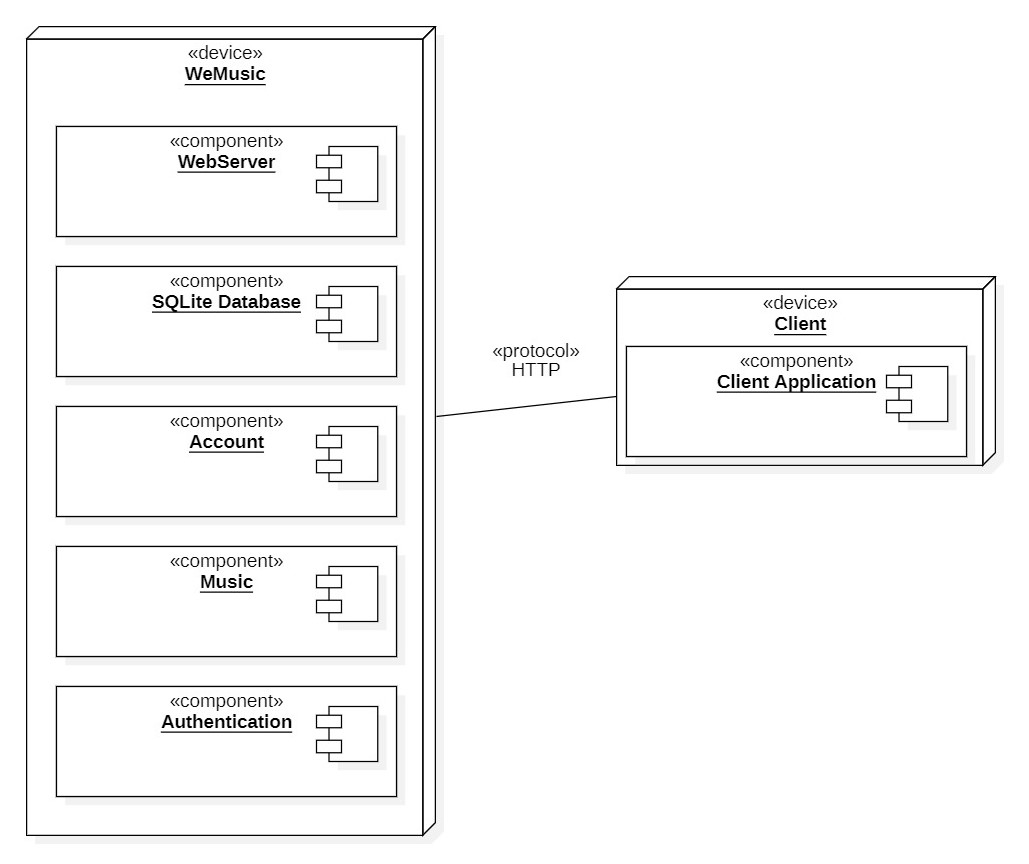
\includegraphics[width=\textwidth]{DeploymentDiagram_ver0.jpg}
    \caption{Deployment Diagram}
    \label{dep_diagram}
\end{figure}


\newpage
\section{Toolchain e tecnologie utilizzate}
\begin{itemize}
      \item \textbf{Modellazione:} Star UML  (Use Case Diagram, Deployment Diagram); diagram.net (Component Diagram, Class Diagram). 
      \item \textbf{Implementazione -- lato client-server:} Django, Bootstrap.
      \item \textbf{Implementazione -- parte dati db:} SQLite.
      \item \textbf{Documentazione, versioning e organizzazione del team:} Latex, GitHub, Discord.
\end{itemize}
\chapter{Iterazione 1}
\section{Introduzione}
Durante la prima iterazione sono state identificate le componenti dal modello dei casi d'uso, 
applicando le euristiche di early design: viene perfezionata la specifica dei componenti 
progettati durante l'iterazione 0 al fine di da definire meglio l'architettura software. 
È stato costruito lo scheletro dell'applicazione tramite la specifica delle differenti classi 
popolate nelle seguenti iterazioni.

Inizialmente, durante lo sviluppo dell'iterazione 0, il sistema nella sua totalità è stato 
visualizzato come una unica componente e sono stati 
introdotti gli attori, ognuno dei quali definito come un'entità esterna. In seguito sono stati 
sviluppati tutti i casi d'uso che riassumono il funzionamento del sistema, i quali vengono, 
nella prima iterazione, raccolti e raggruppati secondo un preciso criterio e affinità. 

Vengono inoltre introdotti componenti e sottocomponenti di controllo di ciascun gruppo, o 
alternativamente componenti di dati; per ognuno di essi nascono parallelamente le classi 
candidate e le relazioni che le legano. 

Per ogni caso d'uso che ha una interazione diretta con un attore esterno viene introdotta 
un'interfaccia per le operazioni visibili esternamente, ovvero le API, offerte o richieste 
dal componente o sottocomponente corrispondente, in base alla direzione dell'interazione. 

Ogni variabile input/output da un attore, specificata nella descrizione di un caso d'uso, 
definisce un parametro di input/di ritorno dell'operazione dell'interfaccia corrispondente. 

Viene quindi scomposto il sistema in sottosistemi e componenti, applicando pattern e 
stili architetturali, per poi distribuire le componenti su nodi computazionali basati su 
uno sviluppo fisico del sistema.


E' necessario specificare che l'architettura di Django si basa sul design pattern \textbf{MVC}, acronimo di Model View 
Controller. Lo scopo di questa scelta di design è la suddivisione della logica in 
tre parti fondamentali favorendo modularità, sviluppo collaborativo e riutilizzo del 
codice oltre a rendere l'applicazione più flessibile e scalabile.
    
Django interpreta il pattern MVC a modo suo, in modo tale che il Controller risulti in 
realtà il framework in sé, le View non scelgano come i dati vadano mostrati bensì quali 
dati mostrare e il come mostrarli viene in realtà deciso nei Template.

Siccome la parte del Controller è gestita dal framework e la View è rappresentata dai Template, Django 
utilizza un framework MTV, ovvero \textbf{Model Template View}.
    
\begin{comment}
Per prima cosa quando viene effettuata una richiesta HTTP essa viene confrontata con gli URL, 
che sono una “mappa” delle risorse disponibili. La richiesta viene quindi inoltrata alla View 
che la gestisce producendo una risposta HTTP della cui formattazione si occuperanno i template, 
mentre il Model fornirà la logica per accedere ai dati e convertirli in tabelle nel database. 

\end{comment}
   
\begin{itemize}
    \item \textbf{M - Model:} “data access layer” - Definisce la struttura delle entità (le classi) del nostro sito, tradotte 
    poi in tabelle nel database.
    \item \textbf{T - Template:} “presentation layer” - Descrive come i dati vadano mostrati nelle pagine web.
    \item \textbf{V - View:} “business logic layer” - Gestisce le richieste e le risposte HTTP, dispone della 
    logica per sapere a quali dati accedere tramite i model e delega la formattazione della risposa ai template, contenendo quindi i metodi. 
\end{itemize}
    
    
\newpage

\section{Casi d'uso}
I casi d'uso vengono raggruppati in tre macro categorie in base a un criterio di affinità:
i primi sono relativi all'autenticazione dell'utente, i secondi sono relativi a tutto
ciò che riguarda l'ambito musicale, ed infine quelli relativi all'account personale e lato social. 
Di seguito un elenco dettagliato dei casi d'uso suddivisi come anticipato.

\subsection{Autenticazione}
    \begin{itemize}
        \item \textbf{UC1:} Sign up 
        \item \textbf{UC2:} Sign in
        \item \textbf{UC3:} Sign out 
    \end{itemize}


\subsection{Musica}
\begin{itemize}
    \item \textbf{Brano:} in questa sezione rientrano tutti i casi d'uso relativi ai brani.
    \begin{itemize}
        \item \textbf{UC4:} Cerca brano
        \item \textbf{UC5:} Cerca album
        \item \textbf{UC6:} Cerca Artista
        \item \textbf{UC7:} Scarica brano
        \item \textbf{UC8:} Like al brano
        \item \textbf{UC19:} ``Discover'' 
    \end{itemize} 
    
    \item \textbf{Playlist:} in questa sezione rientrano tutti i casi d'uso relativi alla creazione e gestione delle playlist.
    \begin{itemize}
        \item \textbf{UC9:} Aggiungi brano a playlist
        \item \textbf{UC15:} Visualizza playlist 
        \item \textbf{UC16:} Crea nuova playlist 
        \item \textbf{UC17:} Elimina playlist
        \item \textbf{UC18:} Modifica playlist
    \end{itemize}
    
    \item \textbf{Artista:} in questa sezione rientrano tutti i casi d'uso relativi alla gestione del profilo artista.
    \begin{itemize}
        \item  \textbf{UC20:} Crea pagina artista 
        \item  \textbf{UC21:} Visualizza pagina artista 
        \item  \textbf{UC22:} Aggiungi brano 
        \item  \textbf{UC23:} Aggiungi album 
        \item  \textbf{UC24:} Personalizza pagina artista 
        \item  \textbf{UC25:} Consulta anagrafica
    \end{itemize} 
\end{itemize}

\subsection{Account}
\begin{itemize}
    \item \textbf{Personale:} in questa sezione rientrano tutti i casi d'uso relativi alla gestione delle informazioni nel proprio profilo personale.
    \begin{itemize}
        \item \textbf{UC12:} Visualizza informazioni profilo 
        \item \textbf{UC13:} Modifica profilo 
        \item \textbf{UC14:} Elimina profilo 
    \end{itemize}
    
    \item \textbf{Amici:} in questa sezione rientrano tutti i casi d'uso relativi alla parte social.
    \begin{itemize}
        \item \textbf{UC10:} Cerca Utente 
        \item \textbf{UC11:} Aggiungi Utente 
    \end{itemize}
\end{itemize}






\newpage

\section{UML Data Class Diagram}
Il Class Diagram in UML permette di descrivere il sistema 
visualizzando i diversi tipi di oggetti all'interno di esso e le relazioni 
statiche che esistono fra loro: sono descritte in maniera più approfondita 
le tre componenti già precedentemente analizzate, ovvero Account, Musica, 
Autenticazione e Discover.
In questo caso viene rappresentato in unico diagramma il Data Class Diagram, 
il quale descrive le classi che compongono la struttura dell'applicazione e le
le entità presenti al suo interno, e il Package/IF Diagram, quindi sono stati
inserite le funzioni implementate. 
nel sistema.
\begin{figure}[H]
    \centering
    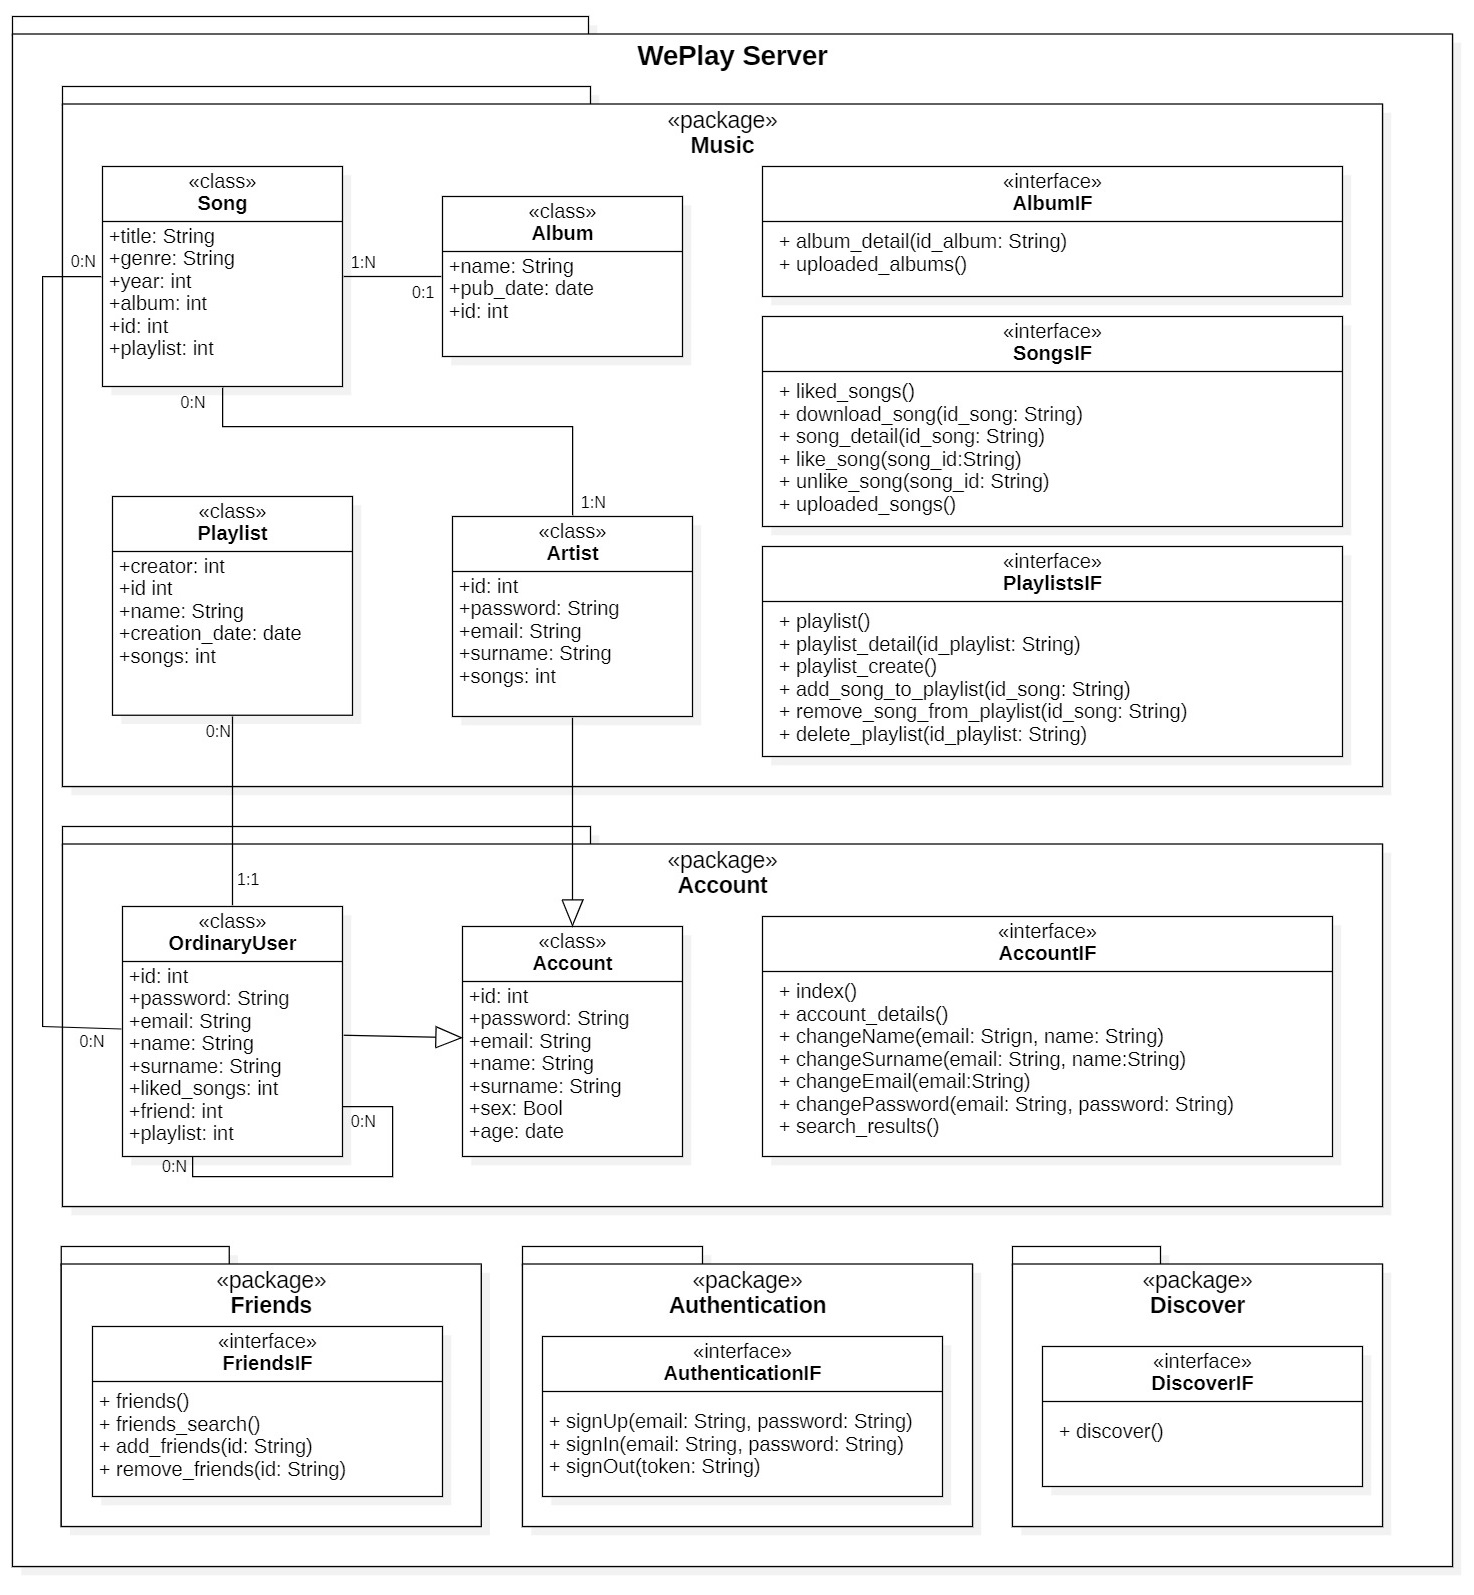
\includegraphics[scale=0.4]{images/ClassDiagram_ver6.jpg}
    \caption{UML Class Diagram}
    \label{fig-uml-class-diag}
\end{figure}
\newpage

\section{UML Component Diagram}
Il Component Diagram in UML ha come obiettivo quello di mostrare la struttura
del sistema software, descrivendo i singoli componenti, le relative interfacce 
e le dipendenze. 

\vspace{2cm}
\subsection{Black Box - Top level}
La rappresentazione black box del sistema è stata gestita partendo da una
una componente centrale, il server del sistema, alla quale si collegano il database e la parte front-end.
Le componenti principali sono: Account, Authentication, Music (che include Brani, Playlist, Album),
Discover e Friends.
\begin{figure}[H]
    \centering
    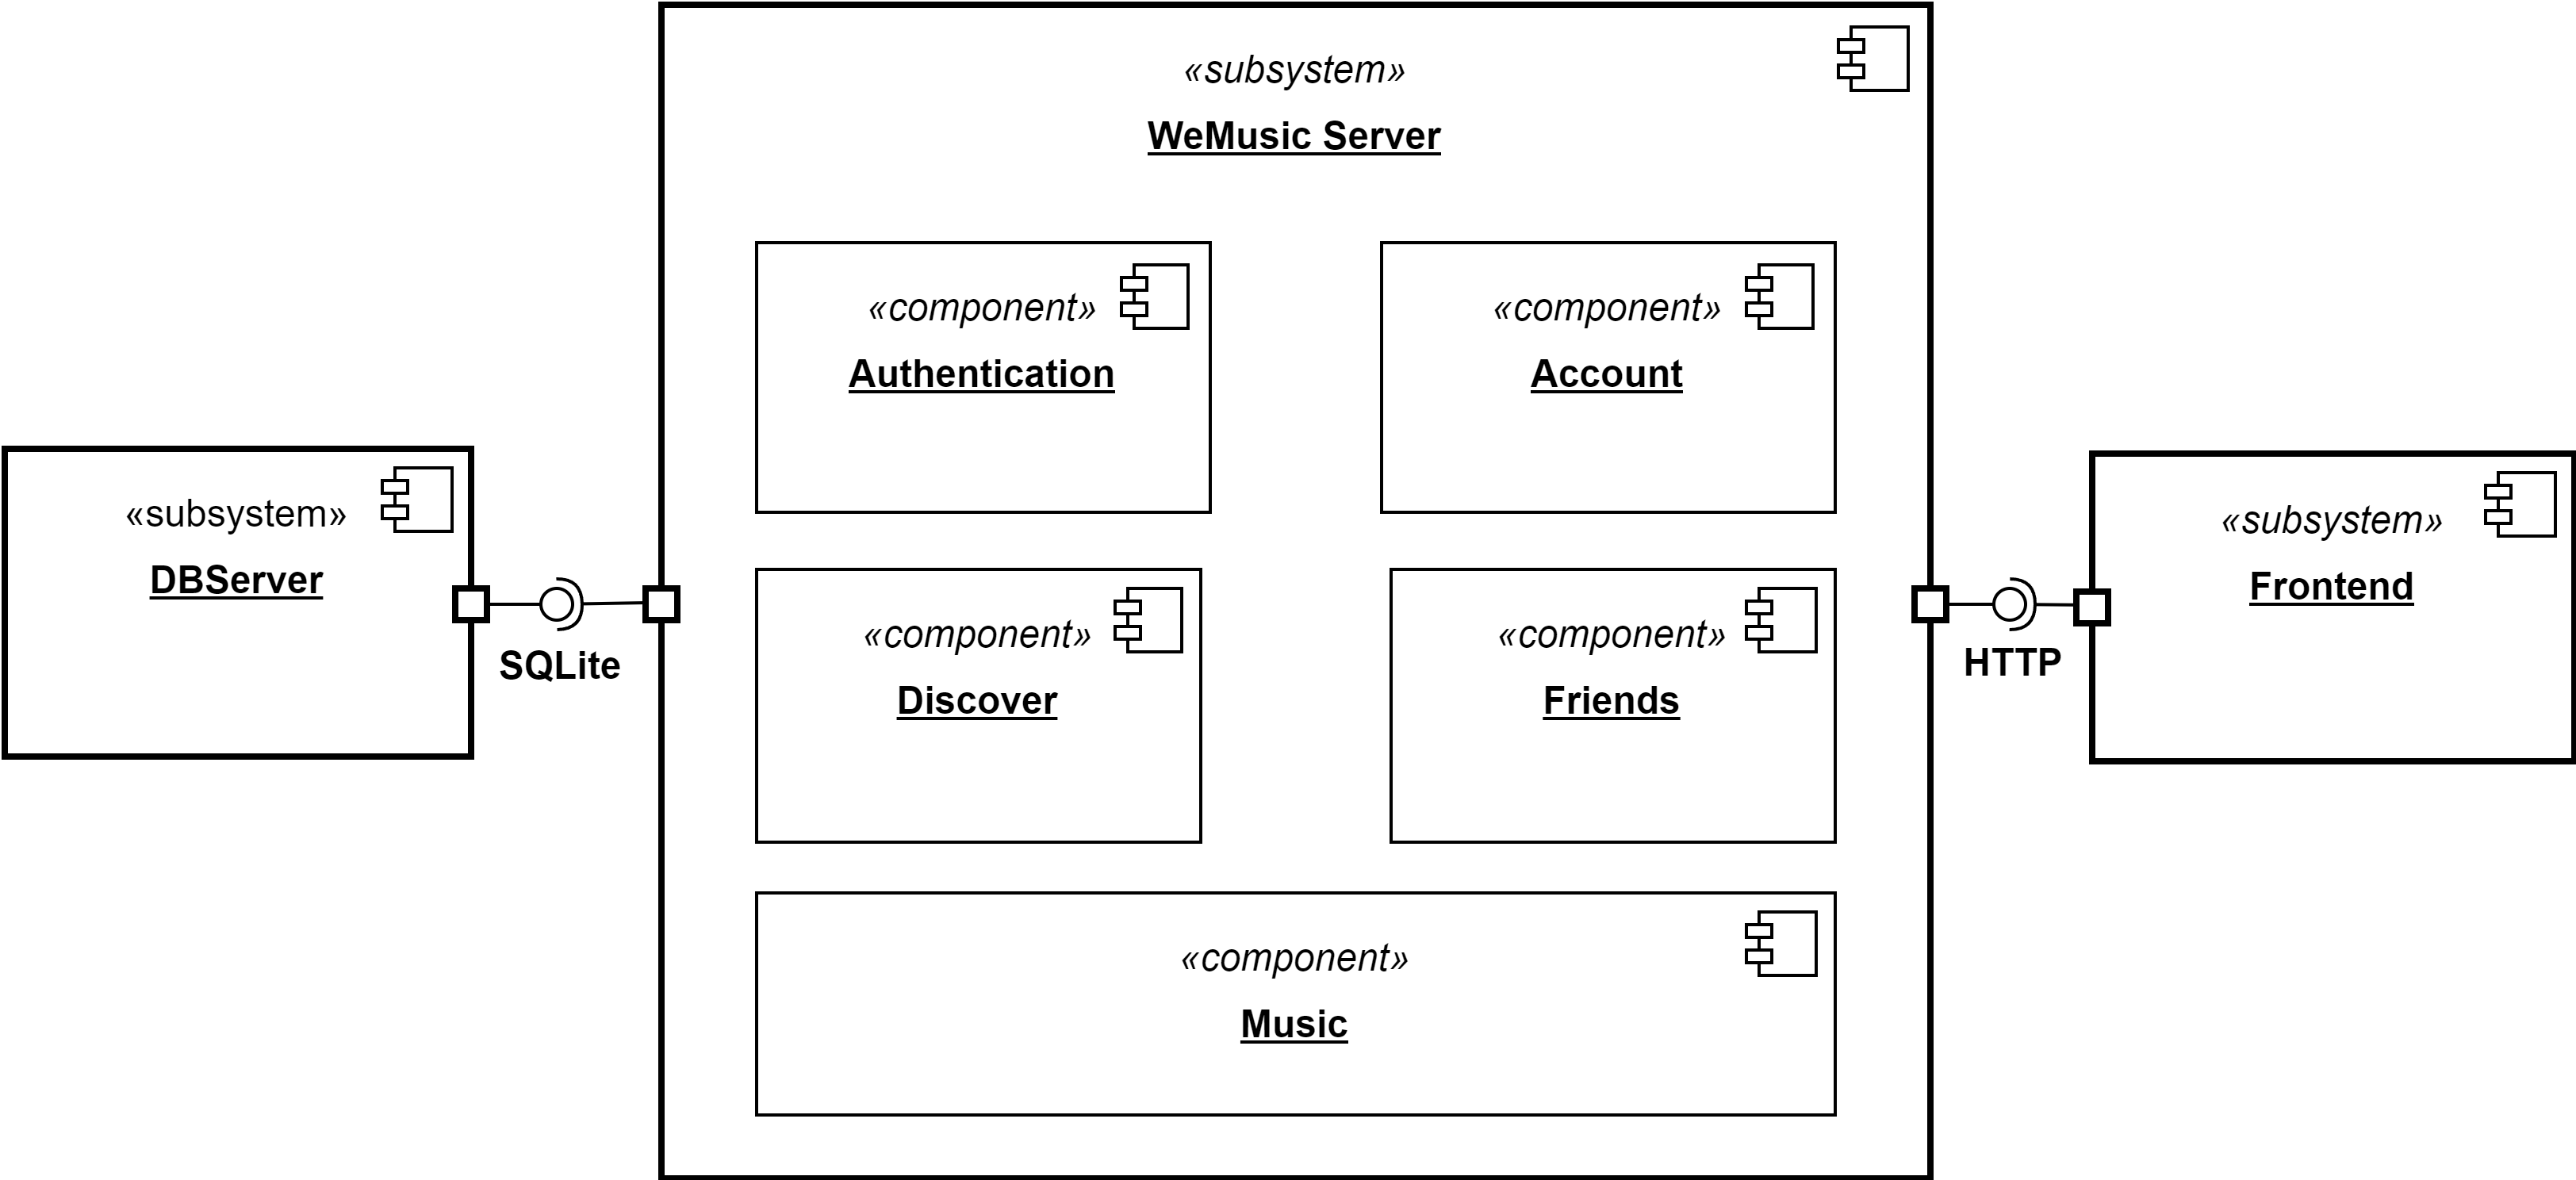
\includegraphics[scale=0.65]{component_diagram_ver4_1.png}
    \caption{UML Component Diagram}
    \label{fig-uml-component-diag_1}
\end{figure}

\newpage
\subsection{White Box - Top level}
La rappresentazione white box del sistema rappresenta anche le componenti
interne e le interfacce tramite le quali comunicano tra loro.

\begin{figure}[H]
    \centering
    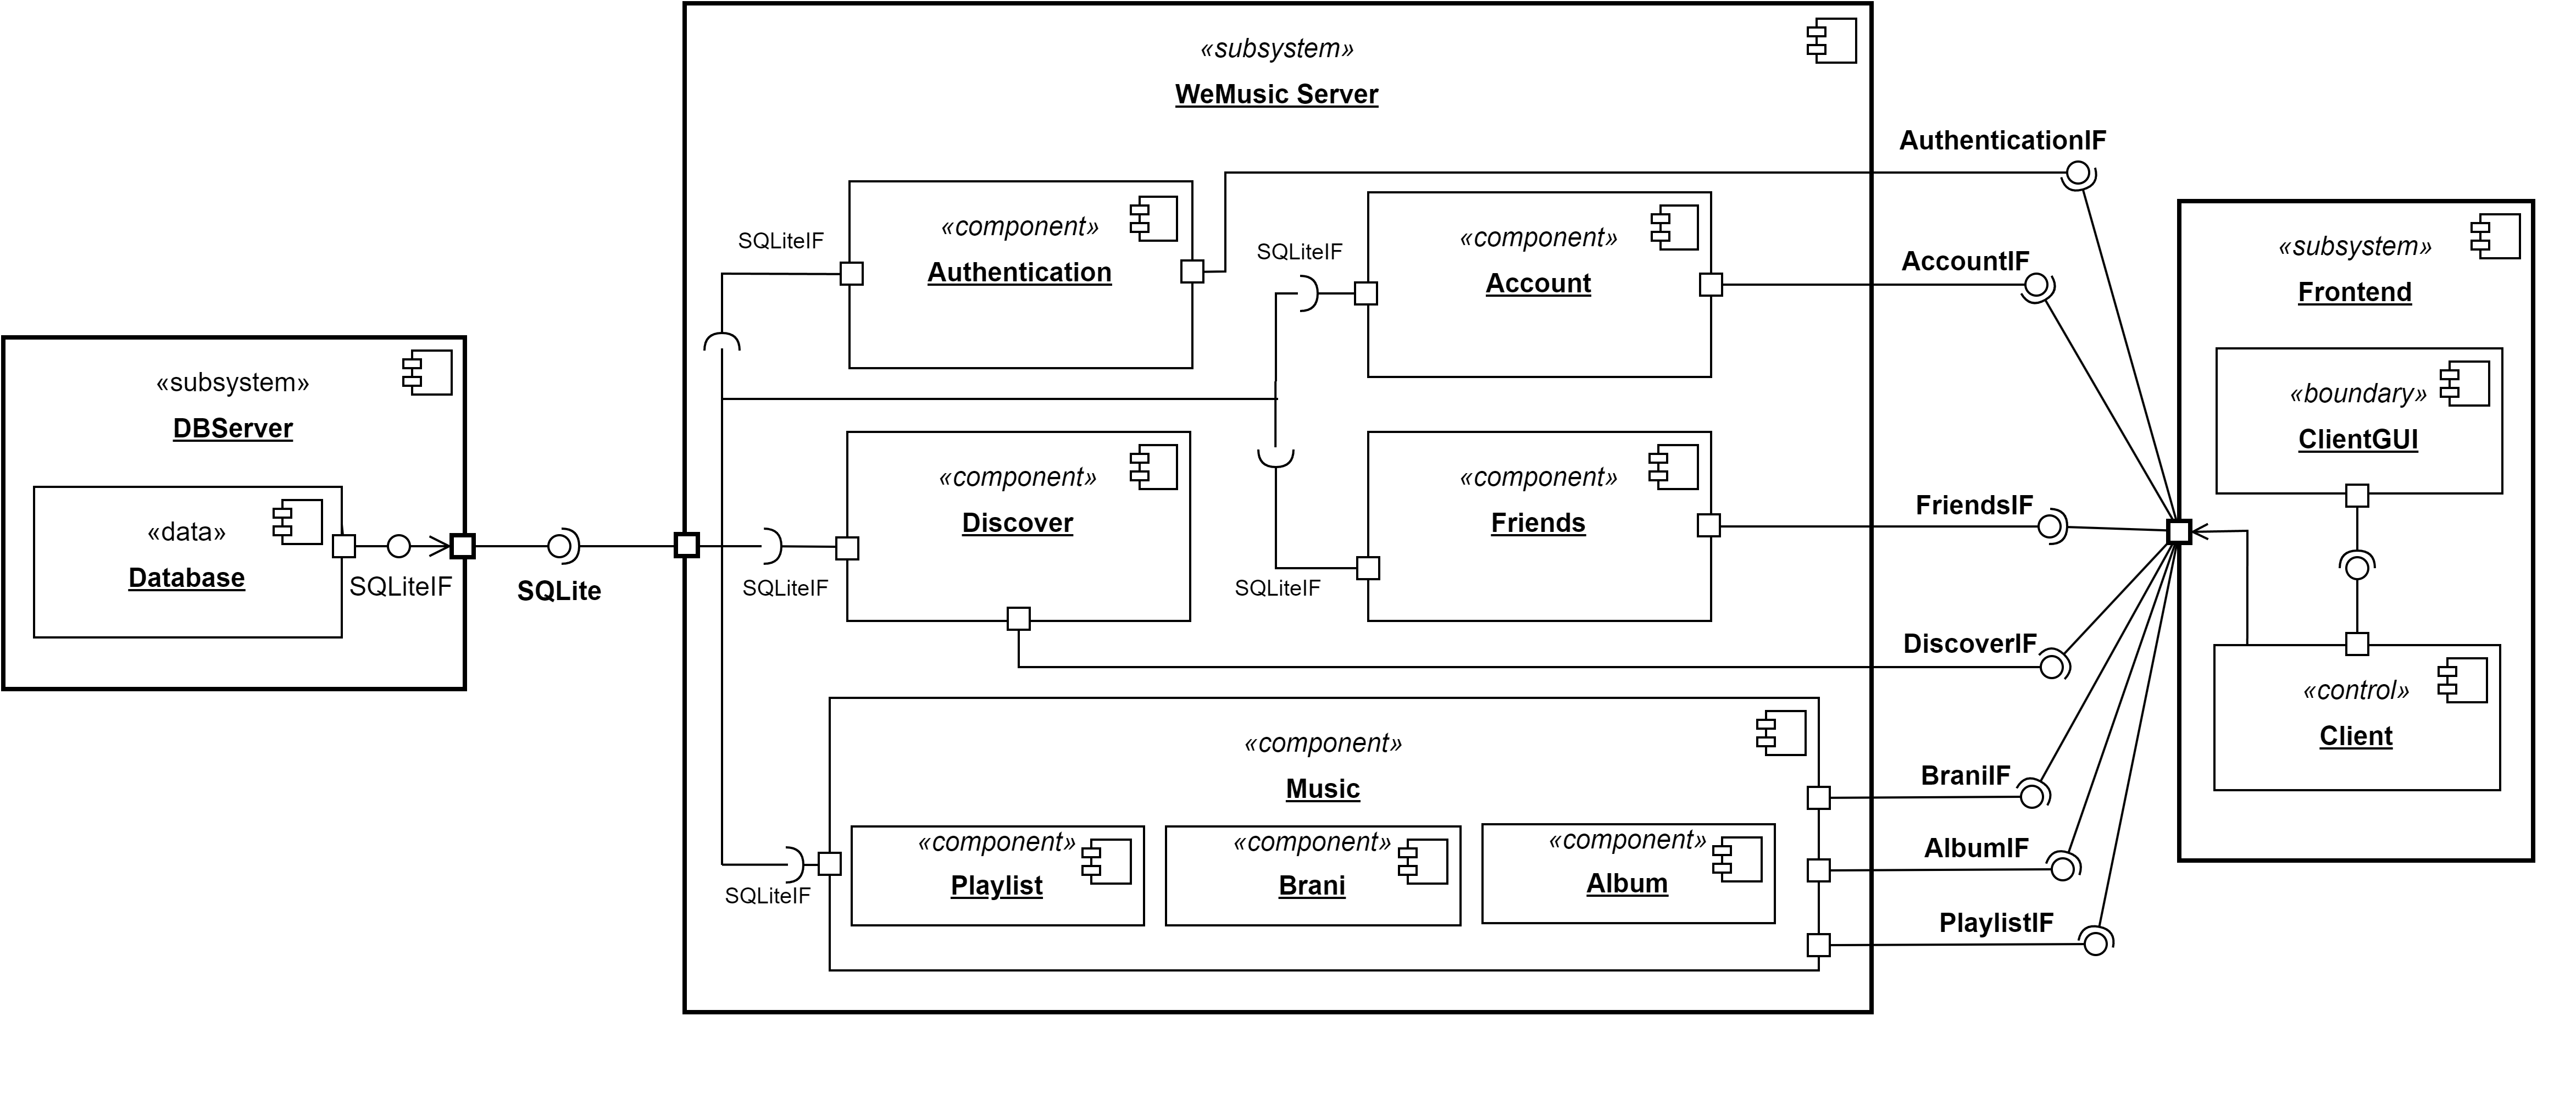
\includegraphics[scale=0.13]{component_diagram_ver4_2.png}
    \caption{UML Component Diagram}
    \label{fig-uml-component-diag_2}
\end{figure}



\chapter{Iterazione 2}
\section{Introduzione}
Nella secconda iterazione sono stati implementati la maggior parte dei casi d'uso: viene proposta 
un'analisi dettagliata di ognuno al fine di specificare gli attori coinvolti nel caso d'uso, l'esecuzione
standard dello stesso, le eventuali precondizioni e le postcondizioni, le eccezioni.
In seguito si procede al testing, quindi analisi statica e dinamica tramite(...)


\newpage
\section{Implementazione}
Di seguito sono elencati i casi d'uso implementati nel sistema WeMusic. Si offre, per ognuno, una breve descrizione dello stesso 
al fine di riassumere la sua funzionalità; inoltre è evidenziato il flow di esecuzione del sito e le varie alterntive che si propongono nel modello.
Infine, vengono specificate eventuali informazioni relative a precondizioni, post condizioni e trigger dello stesso, e le possibili eccezioni nel 
caso avvenga una esecuzione scorretta. 
Seguendo la modellazione proposta in seguito, i casi d'uso relativi all'Autenticazione sono stati completamente implementati, come anche 
la maggior parte di quelli facenti parte del gruppo Musica e Amici. 

\vspace{1cm}
\subsection{UC1 -- Sign up}
Il caso d'uso di Sign up consente all'utente di registrare al sito 
e di poter usufruire dei servizi offerti dallo stesso. 
\begin{itemize}
    \item \textbf{Actor:} Utente base, Artista.
    \item \textbf{Precondition:} Nessuna.
    \item \textbf{Postcondition:} L'utente è registrato al sito, le sue informazioni vengono salvate nel database.
    \item \textbf{Base Sequence:} 
        \begin{itemize}
            \item \textbf{1.} L'utente inserisce nome utente e password.
            \item \textbf{2.} L'utente inserisce i generi preferiti.
            \item \textbf{3.} L'utente ha completato la registrazione.
        \end{itemize}
    \item \textbf{Exception Sequence:} Il nome utente scelto non è valido o è già in uso, o connessione fallita.
        \begin{itemize}
            \item Nel caso di nome utente non valido o già in uso si ritorna al passo 1 della Base Sequence del presente caso d'uso.
            \item Nel caso di connessione fallita si ritorna al passo 1 della Base Sequence del presente caso d'uso. 
        \end{itemize}
    
\end{itemize}
\vspace{1cm}

\subsection{UC2 -- Sign in}
Il caso d'uso di Sign in permette ad un utente già registrato nel sistema di accedere e di poter 
usufruire dei servizi offerti dallo stesso.
\begin{itemize}
    \item \textbf{Actor:} Utente base, Artista.
    \item \textbf{Precondition:} L'utente deve essere già registrato.
    \item \textbf{Postcondition:} L'utente ha effettuato il log in perciò puo navigare la Home page del sito.
    \item \textbf{Base Sequence:}
    \begin{itemize}
        \item \textbf{1.} L'utente inserisce nome utente e password.
        \item \textbf{2.} L'utente clicca sul pulsante di log in.
        \item \textbf{3.} L'utente ha effettuato correttamente l'accesso.
    \end{itemize}
    \item \textbf{Exception Sequence:} La password inserita è errata o connessione fallita.
    \begin{itemize}
        \item Nel caso di password errata si ritorna al passo 1 della Base Sequence del presente caso d'uso.
        \item Nel caso di connessione fallita si ritorna al passo 1 della Base Sequence del caso d'uso \textbf{UC1}.
    \end{itemize}
\end{itemize}

\vspace{1cm}

\subsection{UC3 -- Sign out}
Il caso d'uso di Sign out permette all'utente di disconnettere il 
proprio profilo personale dal sistema.
\begin{itemize}
    \item \textbf{Actor:} Utente base, Artista.
    \item \textbf{Precondition:} L'utente deve essere registrato e deve aver 
        effettuato il log in.
    \item \textbf{Postcondition:} L'utente ha effettuato il log out, perciò non ha più accesso al sistema fino al log in.
    \item \textbf{Base Sequence:}
    \begin{itemize}
        \item \textbf{1.} L'utente clicca il pulsante di Log out nell'interfaccia.
        \item \textbf{2.} L'utente è disconnesso.
    \end{itemize}
    \item \textbf{Exception Sequence:} Connessione fallita.
    \begin{itemize}
        \item Nel caso di connessione fallita si ritorna al passo 1 della Base Sequence del caso d'uso \textbf{UC1}.
    \end{itemize}
\end{itemize}
\vspace{1cm}

\subsection{UC4 -- Cerca brano}
Il caso d'uso di Cerca brano permette di cercare un brano specifico dalla barra di ricerca
tramite precise parole chiave, al fine di scaricarlo per poi riprodurlo in locale.
\begin{itemize}
    \item \textbf{Actor:} Utente base.
    \item \textbf{Precondition:} L'utente deve aver effettuato il log in.
    \item \textbf{Postcondition:} L'utente ha cercato il brano, può dunque mettere like, 
    aggiungerlo ad una playlist personale o scaricarlo. L'utente può scaricare il brano 
    \textbf{(UC7)}, mettere like al brano \textbf{(UC8)}, aggiungerlo ad una playlist \textbf{(UC9)}.
    \item \textbf{Base Sequence:}
    \begin{itemize}
        \item \textbf{1.} L'utente clicca sulla barra di ricerca apposita nell'interfaccia.
        \item \textbf{2.} L'utente digita delle parole chiave per cercare il brano: titolo del brano, album, artista.
        \item \textbf{3.} L'utente ha correttamente eseguito la ricerca: può navigare fra i risultati e selezionare il brano desiderato.
    \end{itemize}
    \item \textbf{Exception Sequence:} Non esiste un brano che corrisponde ai criteri di ricerca o connessione fallita.
    \begin{itemize}
        \item Nel caso di ricerca fallita si ritorna al caso 2 della Base Sequence del presente caso d'uso.
        \item Nel caso di connessione fallita si ritorna al passo 1 della Base Sequence del caso d'uso \textbf{UC1}.
    \end{itemize}
\end{itemize}
\vspace{1cm}

\subsection{UC5 -- Cerca album}
Il caso d'uso di Cerca album consiste nel cercare un album specifico dalla barra di ricerca
tramite precise parole chiave, al fine di selezionare un brano al suo interno e scaricarlo per poi riprodurlo in locale.
\begin{itemize}
    \item \textbf{Actor:} Utente base.
    \item \textbf{Precondition:} L'utente deve aver effettuato il log in.
    \item \textbf{Postcondition:} L'utente ha cercato l'album, può dunque navigare fra i brani che 
    include lo stesso. L'utente può navigare fra i brani dell'album e scaricarli \textbf{(UC7)}, 
    mettere like \textbf{(UC8)}, aggiungerli ad una playlist \textbf{(UC9)}.
    \item \textbf{Base Sequence:}
    \begin{itemize}
        \item \textbf{1.} L'utente clicca sulla barra di ricerca apposita nell'interfaccia.
        \item \textbf{2.} L'utente digita delle parole chiave per cercare l'album: titolo dell'album, artista.
        \item \textbf{3.} L'utente ha correttamente eseguito la ricerca: può navigare fra i risultati e selezionare l'album desiderato.
    \end{itemize}
    \item \textbf{Exception Sequence:} Non esiste un album che corrisponde ai criteri di ricerca o connessione fallita.
    \begin{itemize}
        \item Nel caso di ricerca fallita si ritorna al caso 2 della Base Sequence del presente caso d'uso.
        \item Nel caso di connessione fallita si ritorna al passo 1 della Base Sequence del caso d'uso \textbf{UC1}.
    \end{itemize}
\end{itemize}
\vspace{1cm}

\subsection{UC6 -- Cerca artista}
Il presente caso d'uso consiste nel cercare un artista specifico dalla barra di ricerca
tramite precise parole chiave, al fine di selezionare un brano da lui pubblicato e scaricarlo per poi riprodurlo in locale.
\begin{itemize}
    \item \textbf{Actor:} Utente base.
    \item \textbf{Precondition:} L'utente deve aver effettuato il log in. 
    \item \textbf{Postcondition:} L'utente ha cercato l'artista, può dunque navigare nella pagina 
    artista e scaricare i brani di interesse. L'utente può navigare fra i brani dell'artista e 
    scaricarli \textbf{(UC7)}, mettere like \textbf{(UC8)}, aggiungerli ad una playlist \textbf{(UC9)}.
    \item \textbf{Base Sequence:}
    \begin{itemize}
        \item \textbf{1.} L'utente clicca sulla barra di ricerca apposita nell'interfaccia.
        \item \textbf{2.} L'utente digita delle parole chiave per cercare l'artista, ovvero il nome dell'artista.
        artista.
        \item \textbf{3.} L'utente ha correttamente eseguito la ricerca: può navigare fra i risultati e selezionare l'artista desiderato.
    \end{itemize}
    \item \textbf{Exception Sequence:} Non esiste un artista che corrisponde ai criteri di ricerca o connessione fallita.
    \begin{itemize}
        \item Nel caso di ricerca fallita si ritorna al caso 2 della Base Sequence del presente caso d'uso.
        \item Nel caso di connessione fallita si ritorna al passo 1 della Base Sequence del caso d'uso \textbf{UC1}.
    \end{itemize}
\end{itemize}
\vspace{1cm}

\subsection{UC7 -- Scarica brano}
Il presente caso d'uso consiste nello scaricare un brano al fine di poterlo riprodure in locale.
\begin{itemize}
    \item \textbf{Actor:} Utente base.
    \item \textbf{Precondition:} L'utente deve aver effettuato il log in e individuato il brano desiderato. 
    \item \textbf{Postcondition:} L'utente ha scaricato il brano scelto, quindi può ascoltarlo offline. 
    \item \textbf{Base Sequence:} 
    \begin{itemize}
        \item \textbf{1.} L'utente seleziona il brano desiderato (da una playlist, dalla ricerca, ecc).
        \item \textbf{2.} L'utente clicca sul pulsante di download.
        \item \textbf{3.} L'utente attende il completamento del download.
        \item \textbf{4.} L'utente ha correttamente scaricato il brano.
    \end{itemize}
    \item \textbf{Exception Sequence:} Connessione fallita.
    \begin{itemize}
        \item Nel caso di connessione fallita si ritorna al passo 1 della Base Sequence del caso d'uso \textbf{UC1}.
    \end{itemize}
\end{itemize}
\vspace{1cm}

\subsection{UC8 -- Like al brano}
Il presente caso d'uso consiste nel mettere like ad un brano; in questo modo 
è visibile nell'elenco dei propri brani preferiti.
\begin{itemize}
    \item \textbf{Actor:} Utente base.
    \item \textbf{Precondition:} L'utente deve aver effettuato il log in e individuato il brano desiderato.
    \item \textbf{Postcondition:} L'utente ha aggiunto il brano ai suoi preferiti, quindi può visualizzarlo nell'elenco dei propri preferiti.
    \item \textbf{Base Sequence:}
    \begin{itemize}
        \item \textbf{1.} L'utente seleziona il brano desiderato (da una playlist, dalla ricerca, ecc).
        \item \textbf{2.} L'utente clicca sul pulsante di like.
        \item \textbf{3.} L'utente ha completato correttamente l'operazione: il brano sarà visibile fra i brani preferiti.
    \end{itemize}
    \item \textbf{Exception Sequence:} Connessione fallita.
    \begin{itemize}
        \item Nel caso di connessione fallita si ritorna al passo 1 della Base Sequence del caso d'uso \textbf{UC1}.
    \end{itemize}
\end{itemize}
\vspace{1cm}

\subsection{UC9 -- Aggiungi brano a playlist}
Il presente caso d'uso consiste nell'aggiungere un brano ad una playlist già esistente.
\begin{itemize}
    \item \textbf{Actor:} Utente base.
    \item \textbf{Precondition:} L'utente deve aver effettuato il log in e deve aver creato almeno una playlist, oltre che individuato il brano desiderato.
    \item \textbf{Postcondition:} L'utente ha aggiunto il brano ad una playlist, perciò selezionandola potrà navigare nell'elenco e decidere di scaricarlo \textbf{(UC7)} o mettere like \textbf{(UC8)}.
    \item \textbf{Base Sequence:}
    \begin{itemize}
        \item \textbf{1.} L'utente seleziona il brano desiderato (da una playlist, dalla ricerca, ecc).
        \item \textbf{2.} L'utente clicca sul pulsante apposito.
        \item \textbf{3.} L'utente seleziona la playlist alla quale aggiungere il brano.
        \item \textbf{4.} L'utente ha correttamente inserito il brano nella playlist.
    \end{itemize}
    \item \textbf{Exception Sequence:} Non è stata creata alcuna playlist dall'utente o connessione fallita.
    \begin{itemize}
        \item Nel caso non sia stata creata ancora nessuna playlist si ritorna al passo 3 del presente caso d'uso. 
        \item Nel caso di connessione fallita si ritorna al passo 1 della Base Sequence del caso d'uso \textbf{UC1}.
    \end{itemize}
\end{itemize}
\vspace{1cm}

\subsection{UC15 -- Visualizza playlist}
Il presente caso d'uso consiste nel visualizzare i brano contenuti in una delle proprie playlist. 
\begin{itemize}
    \item \textbf{Actor:} Utente base.
    \item \textbf{Precondition:} L'utente deve aver effettuato il log in e deve aver creato almeno una playlist.
    \item \textbf{Postcondition:} L'utente può consultare il contenuto della playlist, 
    perciò potrà navigare nell'elenco 
    e decidere di scaricare un brano \textbf{(UC7)} o mettere like \textbf{(UC8)}.
    \item \textbf{Base Sequence:}
    \begin{itemize}
        \item \textbf{1.} L'utente seleziona la playlist desiderata (dall'elenco delle proprie playlist).
        \item \textbf{2.} L'utente clicca sulla playlist.
        \item \textbf{3.} L'utente ha correttamente eseguito l'operazione: può navigare fra i brani contenuti nella playlist.
    \end{itemize}
    \item \textbf{Exception Sequence:} Non è stata creata alcuna playlist dall'utente o connessione fallita.
    \begin{itemize}
        \item Nel caso non sia stata creata ancora nessuna playlist si ritorna al passo 1 del presente caso d'uso.
        \item Nel caso di connessione fallita si ritorna al passo 1 della Base Sequence del caso d'uso \textbf{UC1}.
    \end{itemize}
\end{itemize}
\vspace{1cm}

\subsection{UC16 -- Crea nuova playlist}
Il presente caso d'uso consiste nel creare una nuova playlist al fine di inserire brani al suo interno.
\begin{itemize}
    \item \textbf{Actor:} Utente base.
    \item \textbf{Precondition:} L'utente deve aver effettuato il log in.
    \item \textbf{Postcondition:} L'utente può aggiungere brani alla playlist appena creata \textbf{(UC9)}
    \item \textbf{Base Sequence:}
    \begin{itemize}
        \item \textbf{1.} L'utente seleziona la playlist desiderata (dall'elenco delle proprie playlist).
        \item \textbf{2.} L'utente clicca sulla playlist.
        \item \textbf{3.} L'utente ha correttamente eseguito l'operazione: può navigare fra i brani contenuti nella playlist.
    \end{itemize}
    \item \textbf{Exception Sequence:} Connessione fallita.
    \begin{itemize}
        \item Nel caso di connessione fallita si ritorna al passo 1 della Base Sequence del caso d'uso \textbf{UC1}.
    \end{itemize}
\end{itemize}
\vspace{1cm}

\subsection{UC17 -- Elimina playlist}
Il presente caso d'uso consiste nell'eliminare una delle proprie playlist.
\begin{itemize}
    \item \textbf{Actor:} Utente base.
    \item \textbf{Precondition:} L'utente deve aver effettuato il log in e deve aver creato almeno una playlist.
    \item \textbf{Postcondition:} L'utente ha eliminato la playlist, quindi non sarà più visibile nell'elenco delle proprie playlist.
    \item \textbf{Base Sequence:}
    \begin{itemize}
        \item \textbf{1.} L'utente seleziona la playlist desiderata dall'elenco delle proprie playlist.
        \item \textbf{2.} L'utente clicca su elimina playlist.
        \item \textbf{3.} L'utente ha correttamente eliminato la playlist: essa non sarà più visibile nell'elenco.
    \end{itemize}
    \item \textbf{Exception Sequence:} Non è stata creata alcuna playlist dall'utente o connessione fallita.
    \begin{itemize}
        \item Nel caso non sia stata creata ancora nessuna playlist si ritorna al passo 1 del presente caso d'uso.
        \item Nel caso di connessione fallita si ritorna al passo 1 della Base Sequence del caso d'uso \textbf{UC1}.
    \end{itemize}
\end{itemize}
\vspace{1cm}

\subsection{UC18 -- Modifica playlist}
Il presente caso d'uso consiste nel poter modificare delle proprie playlist: può modificare il nome della stessa o rimuovere un brano da essa.
\begin{itemize}
    \item \textbf{Actor:} Utente base.
    \item \textbf{Precondition:} L'utente deve aver effettuato il log in e deve aver creato almeno una playlist.
    \item \textbf{Postcondition:} L'utente ha modificato con successo la playlist, quindi sarà visualizzato il nuovo nome/i brani eliminati non saranno più nell'elenco.
    \item \textbf{Base Sequence:}
    \begin{itemize}
        \item \textbf{1.} L'utente seleziona la playlist desiderata dall'elenco delle proprie playlist.
        \item \textbf{2.} L'utente clicca su modifica playlist.
        \item \textbf{3.} L'utente modifica il nome/elimina i brani desiderati.
        \item \textbf{4.} L'utente ha modificato con successo la playlist.
    \end{itemize}
    \item \textbf{Exception Sequence:} Non è stata creata alcuna playlist dall'utente o connessione fallita.
    \begin{itemize}
        \item Nel caso non sia stata creata ancora nessuna playlist si ritorna al passo 1 del presente caso d'uso.
        \item Nel caso di connessione fallita si ritorna al passo 1 della Base Sequence del caso d'uso \textbf{UC1}.
    \end{itemize}
\end{itemize}
\vspace{1cm}

\subsection{UC10 -- Cerca Utente}
\begin{itemize}
    \item \textbf{Actor:} Utente base.
    \item \textbf{Precondition:} L'utente deve aver effettuato il log in.
    \item \textbf{Postcondition:} L'utente ha effettuato con successo la ricerca: può aggiungere l'utente fra i propri amici \textbf{(UC11)}
    \item \textbf{Base Sequence:}
    \begin{itemize}
        \item \textbf{1.} L'utente clicca sulla barra di ricerca apposita nell'interfaccia.
        \item \textbf{2.} L'utente digita delle parole chiave per cercare l'utente, ovvero il suo nome e cognome.
        artista.
        \item \textbf{3.} L'utente ha correttamente eseguito la ricerca: può navigare fra i risultati e selezionare l'utente desiderato.
    \end{itemize}
    \item \textbf{Exception Sequence:} Non esiste un utente che corrisponde ai criteri di ricerca o connessione fallita.
    \begin{itemize}
        \item Nel caso di ricerca fallita si ritorna al caso 2 della Base Sequence del presente caso d'uso.
        \item Nel caso di connessione fallita si ritorna al passo 1 della Base Sequence del caso d'uso \textbf{UC1}.
    \end{itemize}
\end{itemize}
\vspace{1cm}

\subsection{UC11 -- Aggiungi Utente}
\begin{itemize}
    \item \textbf{Actor:} Utene base.
    \item \textbf{Precondition:} L'utente deve aver effettuato il log in e aver effettuato correttamente la ricerca.
    \item \textbf{Postcondition:} L'utente ha aggiunto correttamente l'utente desiderato che sarà visibile nella propria lista di amici.
    \item \textbf{Base Sequence:}
    \begin{itemize}
        \item \textbf{1.} L'utente, dopo aver effettuato la ricerca, clicca sull'utente desiderato.
        \item \textbf{2.} L'utente clicca su Aggiungi
        \item \textbf{3.} L'utente ha correttamente aggiunto l'amico.
    \end{itemize}
    \item \textbf{Exception Sequence:} Connessione fallita.
    \begin{itemize}
        \item Nel caso di connessione fallita si ritorna al passo 1 della Base Sequence del caso d'uso \textbf{UC1}.
    \end{itemize}
\end{itemize}
\vspace{1cm}

\subsection{UC12 -- Visualizza informazioni profilo}
\begin{itemize}
    \item \textbf{Actor:} Utente base.
    \item \textbf{Precondition:} L'utente deve aver effettuato il log in.
    \item \textbf{Postcondition:} L'utente ha correttamente eseguito l'operazione: può modificare le proprie informazioni personali \textbf{(UC13)}.
    \item \textbf{Base Sequence:}
    \begin{itemize}
        \item \textbf{1.} L'utente clicca sulle info del proprio profilo.
        \item \textbf{2.} L'utente ha correttamente eseguito l'operazione.
    \end{itemize}
    
    \item \textbf{Exception Sequence:} Connessione fallita.
    \begin{itemize}
        \item Nel caso di connessione fallita si ritorna al passo 1 della Base Sequence del caso d'uso \textbf{UC1}.
    \end{itemize}
\end{itemize}
\vspace{1cm}

\subsection{UC13 -- Modifica profilo}
\begin{itemize}
    \item \textbf{Actor:} Utente base.
    \item \textbf{Precondition:} L'utente deve aver effettuato il log in e visitare la pagina relativa alle informazioni personali.
    \item \textbf{Postcondition:} L'utente ha correttamente modificato il proprio profilo: saranno visualizzate le informazioni personali aggiornate.
    \item \textbf{Base Sequence:}
    \begin{itemize}
        \item \textbf{1.} L'utente, dopo aver visualizzato le info del proprio profilo, clicca su modifica.
        \item \textbf{2.} L'utente effettua le modifiche desiderate.
        \item \textbf{3.} L'utente clicca su Salva modifiche.
        \item \textbf{4.} L'utente ha correttamente eseguito l'operazione.
    \end{itemize}
    \item \textbf{Exception Sequence:} Connessione fallita.
    \begin{itemize}
        \item Nel caso di connessione fallita si ritorna al passo 1 della Base Sequence del caso d'uso \textbf{UC1}.
    \end{itemize}
\end{itemize}
\vspace{1cm}

\subsection{UC14 -- Elimina profilo}
\begin{itemize}
    \item \textbf{Actor:} Utente base, Artista.
    \item \textbf{Precondition:} L'utente deve aver effettuato il log in.
    \item \textbf{Postcondition:} L'utente ha correttamente eliminato il proprio profilo, può registrarsi nuovamente \textbf{(UC1)} per usufruire dei servizi offerti al sistema. 
    \item \textbf{Base Sequence:}
    \begin{itemize}
        \item \textbf{1.} L'utente, dopo aver visualizzato le info del proprio profilo, clicca su elimina profilo.
        \item \textbf{2.} L'utente conferma la decidione.
        \item \textbf{3.} L'utente ha correttamente eseguito l'operazione.
    \end{itemize}
    \item \textbf{Exception Sequence:} Connessione fallita.
    \begin{itemize}
        \item Nel caso di connessione fallita si ritorna al passo 1 della Base Sequence del caso d'uso \textbf{UC1}.
    \end{itemize}
\end{itemize}
\vspace{1cm}

\subsection{UC19 -- ``Discover'' e classifiche}
\begin{itemize}
    \item \textbf{Actor:} Utente base.
    \item \textbf{Precondition:}
    \item \textbf{Postcondition:}
    \item \textbf{Base Sequence:}
    \item \textbf{Branch Sequence:}
    \item \textbf{Exception Sequence:}
    \item \textbf{Sub UseCase:}
\end{itemize}
\vspace{1cm}


\section{Testing}

\chapter{Iterazione 3}
\section{Introduzione}
Nella terza iterazione è stato approfondito e implementato l'algoritmo portante del sistema: l'algoritmo di Discover permette di ``Scoprire" nuova 
musica e nuovi utenti in base alle preferenze dell'utente.

\section{Implementazione del caso d'uso}
\subsection{UC19 -- ``Discover''}
\begin{itemize}
    \item \textbf{Actor:} Utente base.
    \item \textbf{Precondition:} L'utente deve aver effettuato il log in.
    \item \textbf{Postcondition:} L'utente può scoprire nuovi brani e aggiungere nuovi amici secondo i suggerimenti dell'algoritmo. 
    \item \textbf{Base Sequence:}
    \begin{itemize}
        \item \textbf{1.} L'utente, dopo aver effettuato il log in, clicca su Discover dal menu a sinistra.
        \item \textbf{2.} L'utente naviga nella pagina dei brani e amici suggeriti.
        \item \textbf{3.} L'utente ha correttamente eseguito l'operazione.
    \end{itemize}
    \item \textbf{Exception Sequence:} Connessione fallita.
    \begin{itemize}
        \item Nel caso di connessione fallita si ritorna al passo 1 della Base Sequence del caso d'uso \textbf{UC1}.
    \end{itemize}
\end{itemize}
\vspace{1cm}

\section{UML Component Diagram}
In figura sono presenti tutte le interfacce
relative alle componenti implementate in questa iterazione, 
ovvero Amici e Discover (parte relativa all'algoritmo).
\begin{figure}[H]
    \centering
    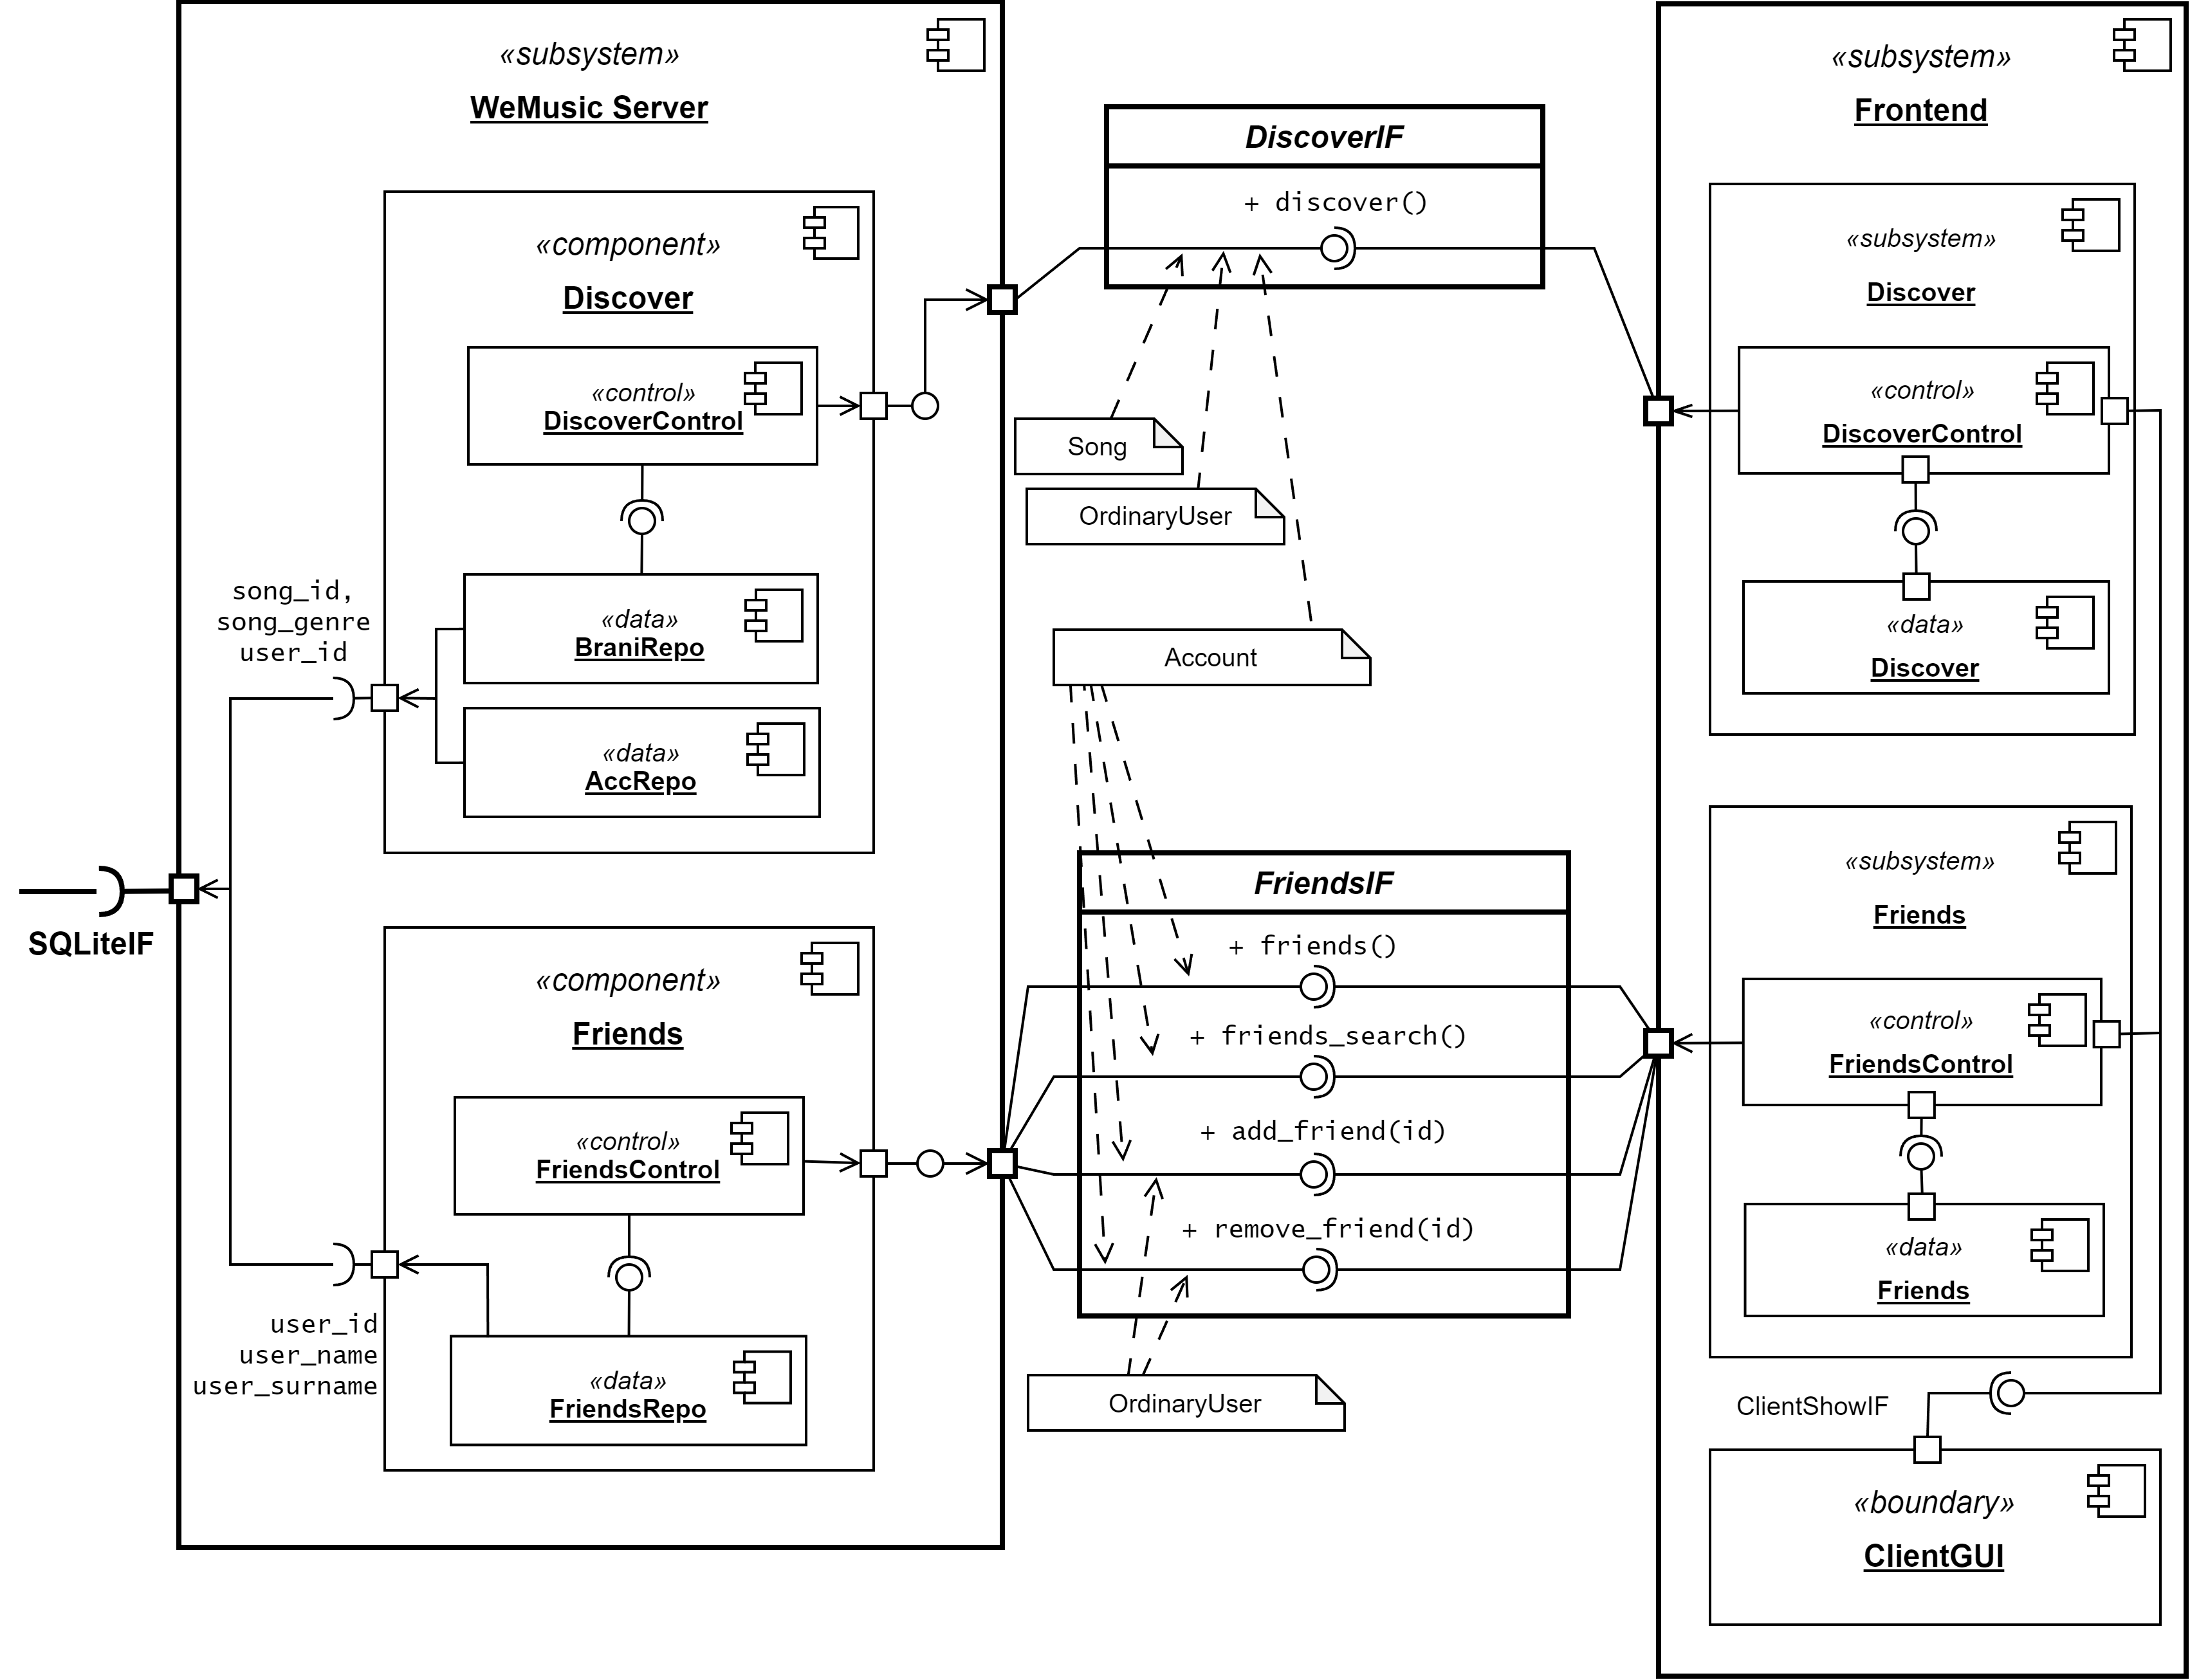
\includegraphics[scale=0.64]{component_diagram_ver5_5.png} 
    \caption{UML Component Diagram}
    \label{fig-uml-component-diag_5}
\end{figure}

\newpage
\section{Descrizione dell'algoritmo}
L'algoritmo di Discover è stato ideato per offrire all'utente un'esperienza completa di riproduzione e scoperta di nuova musica, unendo a ciò la 
componente social: in questo modo si permette all'utente di conoscere nuove persone che condividono con lui i propri gusti musicali. 

Questo tipo di algoritmo 
tiene traccia dei generi preferiti dell'utente e lo utilizza per suggerire musica simile, ma non solo: allo stesso modo riesce a suggerire 
una lista di utenti che hanno gusti simili all'utente loggato, in modo da poterli aggiungere alla propria lista di amici.  

Le variabili e i fattori tenuti in considerazione per lo sviluppo dell'algoritmo di Discover sono i seguenti: 
\begin{itemize}
    \item Il genere favorito dell'utente, ottenuto da un'analisi dei suoi brani preferiti;
    \item L'età dell'utente;
    \item Il sesso dell'utente.
\end{itemize}

\vspace{1cm}
\section{Funzionamento dell'algoritmo}
Il funzionamento dell'algoritmo si basa su una previsione Machine Learning, tramite la libreria \textbf{Pandas} di Python;
il nome fa riferimento sia a ``Panel Data" che ``Python Data Analysis", infatti è una libreria molto utilizzata per lavorare 
con dataset: tramite le sue molteplici funzioni consente di analizzare, pulire, esplorare e manipolare i dati, definendo 
conclusioni basate su teorie statistiche. 

Come anticipato, in base al genere preferito dell'utente, il suo sesso e la sua età, l'algoritmo suggerisce dei brani ricavandoli 
da un dataset, filtrandoli secondo le variabili sopracitate. Al termine dell'esecuzione l'algoritmo mostrerà un elenco di brani e amici suggeriti.

Gli step di funzionamento dell'algoritmo possono essere così riassunti: 
\begin{itemize}
    \item Inizialmente, viene creato un oggetto account contenente le informazioni relative all'account dell'utente loggato, che ci serviranno in seguito; 
    viene passato il parametro \textbf{request} che è quello che contiene le informazioni di interesse, ovvero l'età e il sesso (1=maschio, 0=femmina). 
    In seguito viene utilizzato un training set (\textbf{utenti.csv}) sul quale allenare la stima, contenente le informazioni degli utenti 
    necessarie per estrapolare le variabili: quelle di input includono il sesso e l'età dell'utente, quella di output contiene solo 
    il genere preferito (ciò che suggerirà l'algoritmo). 

    \item Dopo aver creato queste due tabelle viene istanziato il modello previsionale tramite il comando \textbf{DecisionTreeClassifier}, un comando 
    della libreria Pandas che permette, dandogli in input le variabili considerate, di fittare il modello che le lega. 
    
    \item Viene quindi fittato il modello tramite il comando \textbf{modello.fit(...)}, che si allenerà sulle variabili scelte (età e sesso), per restituire 
    il risultato (genere preferito). 

    \item In seguito verrà effettuata la predizione inserendo le informazioni relative all'utente loggato tramite la funzione \textbf{modello.predict}, ed 
    infine viene memorizzata la previsione relativa solo alla variabile di genere musicale. 
    
\end{itemize}

\vspace{1cm}
\subsection{Discover: Suggerimento brano}
Nella parte successiva dell'algoritmo Discover si effettua un semplice filtro su tutte le canzoni presenti nel database del sistema e vengono
 selezionate solo quelle che rispettano il genere target restituito dall'algoritmo Discover; vengono in seguito salvate in una 
 lista e proposte all'utente, che sarà in grado di navigare e selezionare quale scaricare o aggiungere ai preferiti o ad una playlist. 

 
\newpage
\subsection{Discover: Suggerimento amici}
Nell'ultima parte dell'algoritmo Discover viene seguito un processo più meccanico: facendo ancora riferimento al genere target 
individuato nella parte iniziale dell'algoritmo, viene estrapolata una lista di amici suggeriti per l'utente. 

Inizialmente viene creata una lista amici vuota, vengono salvate le informazioni relative dell'utente loggato, vengono quindi 
selezionati tutti gli utenti presenti nella lista amici (in modo da escluderli in seguito nell'algoritmo).
Dopo aver creato una lista degli identificativi, tramite un ciclo for each vengono selezionati gli utenti nel database 
sfogliando per ognuno le canzoni preferite, al fine di salvare il genere di ogni canzone in una variabile y.

Condizione per rientrare negli utenti suggeriti:
\begin{itemize}
    \item L'utente analizzato (nel database) non deve essere l'utente loggato, ovvero devono avere id diversi;
    \item L'utente analizzato (nel database) non deve essere amico dell'utente loggato, ovvero il suo id non deve essere presente 
    nella lista amici;
    \item All'utente analizzato (nel database) deve piacere almeno una canzone che abbia lo stesso genere target dell'algoritmo.

\end{itemize}

Nel context viene poi passata la lista creata con gli utenti selezionati dal database, in modo da permettere all'utente di poter
navigare fra gli utenti ed, eventualmente, aggiungerli fra gli amici. 




\newpage

\section{Studio della complessità}

\subsection{Algortimo Parte I}
\vspace{0.5cm}
\subparagraph{Pseudocodice}
Pseudocodice della prima parte dell'algoritmo, relativa all'inizializzazione 
e all'individuazione del genere target. 
% codice 1
%\begin{figure}[H]
%    \centering
%    \begin{center}
%    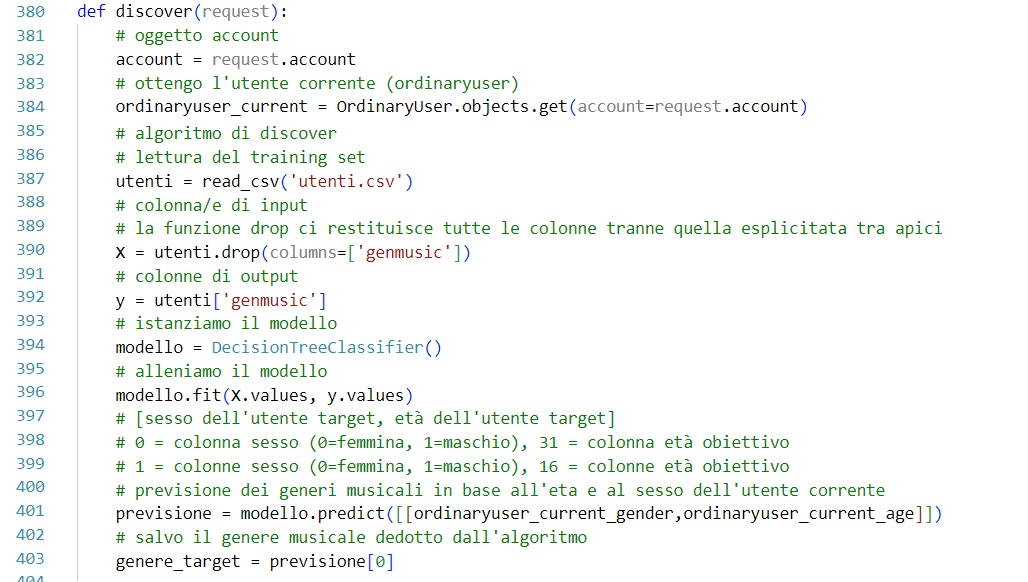
\includegraphics[scale=0.5]{images/alg1_v2.jpg}
%    \end{center}
%    \caption{Codice (parte I)}
%    \label{fig-codice1}
%\end{figure}

% pseudocodice 1
\begin{algorithm}
    \caption{Step 1 - Inizializzazione}
    \SetAlgoLined
    \LinesNumbered
    \SetKwProg{myalg}{algoritmo}{ begin}{end}
    \myalg{Discover($curr\_gender$, $curr\_age$)}{
        \BlankLine
        \BlankLine
        \textbf{/* Creazione oggetto account */}\

        \textbf{do}{
            $account \leftarrow request.account$
        }
        \BlankLine
        \BlankLine
        
        \textbf{/* Memorizzazione utente corrente */}\\
            \textbf{do}{
            $curr\_user \leftarrow curr\_user.\underline{get}()$
        }
        \BlankLine
        \BlankLine
        \textbf{/* Lettura training set degli utenti.csv */}\
            
        \textbf{do}{
           $utenti \leftarrow read\_csv('utenti.csv')$
        }
        \BlankLine
        \BlankLine
        \textbf{/* Creazione colonna di input della previsione */}\
            
        \textbf{do}{
            $X \leftarrow utenti.\underline{drop}(columns=['genmusic'])$
        }
        \BlankLine
        \BlankLine
        \textbf{/* Creazione colonna di output della previsione */}\
            
        \textbf{do}{
            $y \leftarrow utenti['genmusic'] $
        }
        \BlankLine
        \BlankLine
        \textbf{/* Creazione istanza del modello */}\
            
        \textbf{do}{
            $ modello \leftarrow \underline{DecisionTreeClassifier}()$
        }
        \BlankLine
        \BlankLine
        \textbf{/* Allenamento del modello sui dati */}\
            
        \textbf{do}{
            $ modello.\underline{fit}(X.values, y.values)$
        }
        \BlankLine
        \BlankLine
        \textbf{/* Previsione dei generi */}\
            
        \textbf{do}{
            $previsione \leftarrow modello.\underline{predict}(curr\_gender, curr\_age)$
        }
        \BlankLine
        \BlankLine
        \textbf{/* Memorizzazione del genere target */}\

        \textbf{do}{
            $genere\_target \leftarrow previsione[0]$
        } 

        \BlankLine
        \textbf{...}
        \BlankLine
        \KwResult{Genere target}
        \BlankLine
        
    }
\end{algorithm}

% flowchart 1
\newpage

%\subparagraph{Diagramma di flusso} 
%Diagramma di flusso della prima parte dell'algoritmo.
%\begin{figure} [H]
%    \centering
%    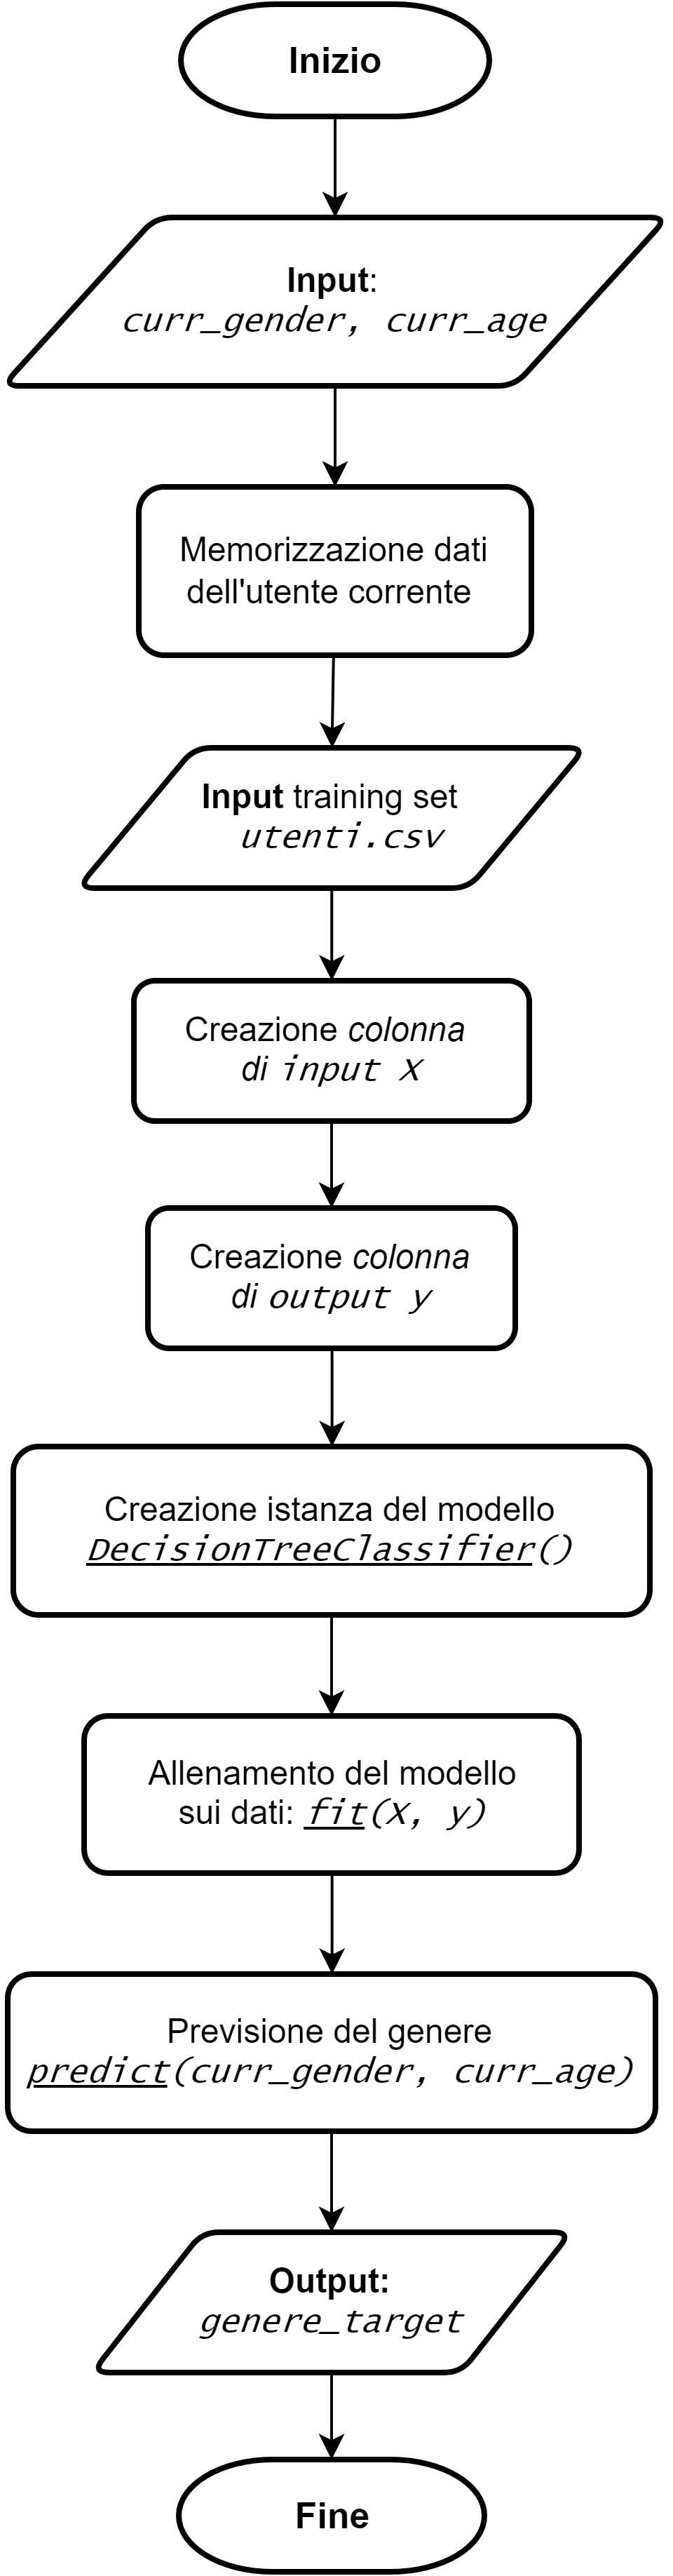
\includegraphics[scale=0.7]{images/flowchart-Parte I.png}
%    \caption{Flowchart (parte I)}
%    \label{fig-fc1}
%\end{figure}

\subparagraph{UML Activity Diagram}
Diagramma delle attività della prima parte dell'algoritmo.
\begin{figure} [H]
    \centering
    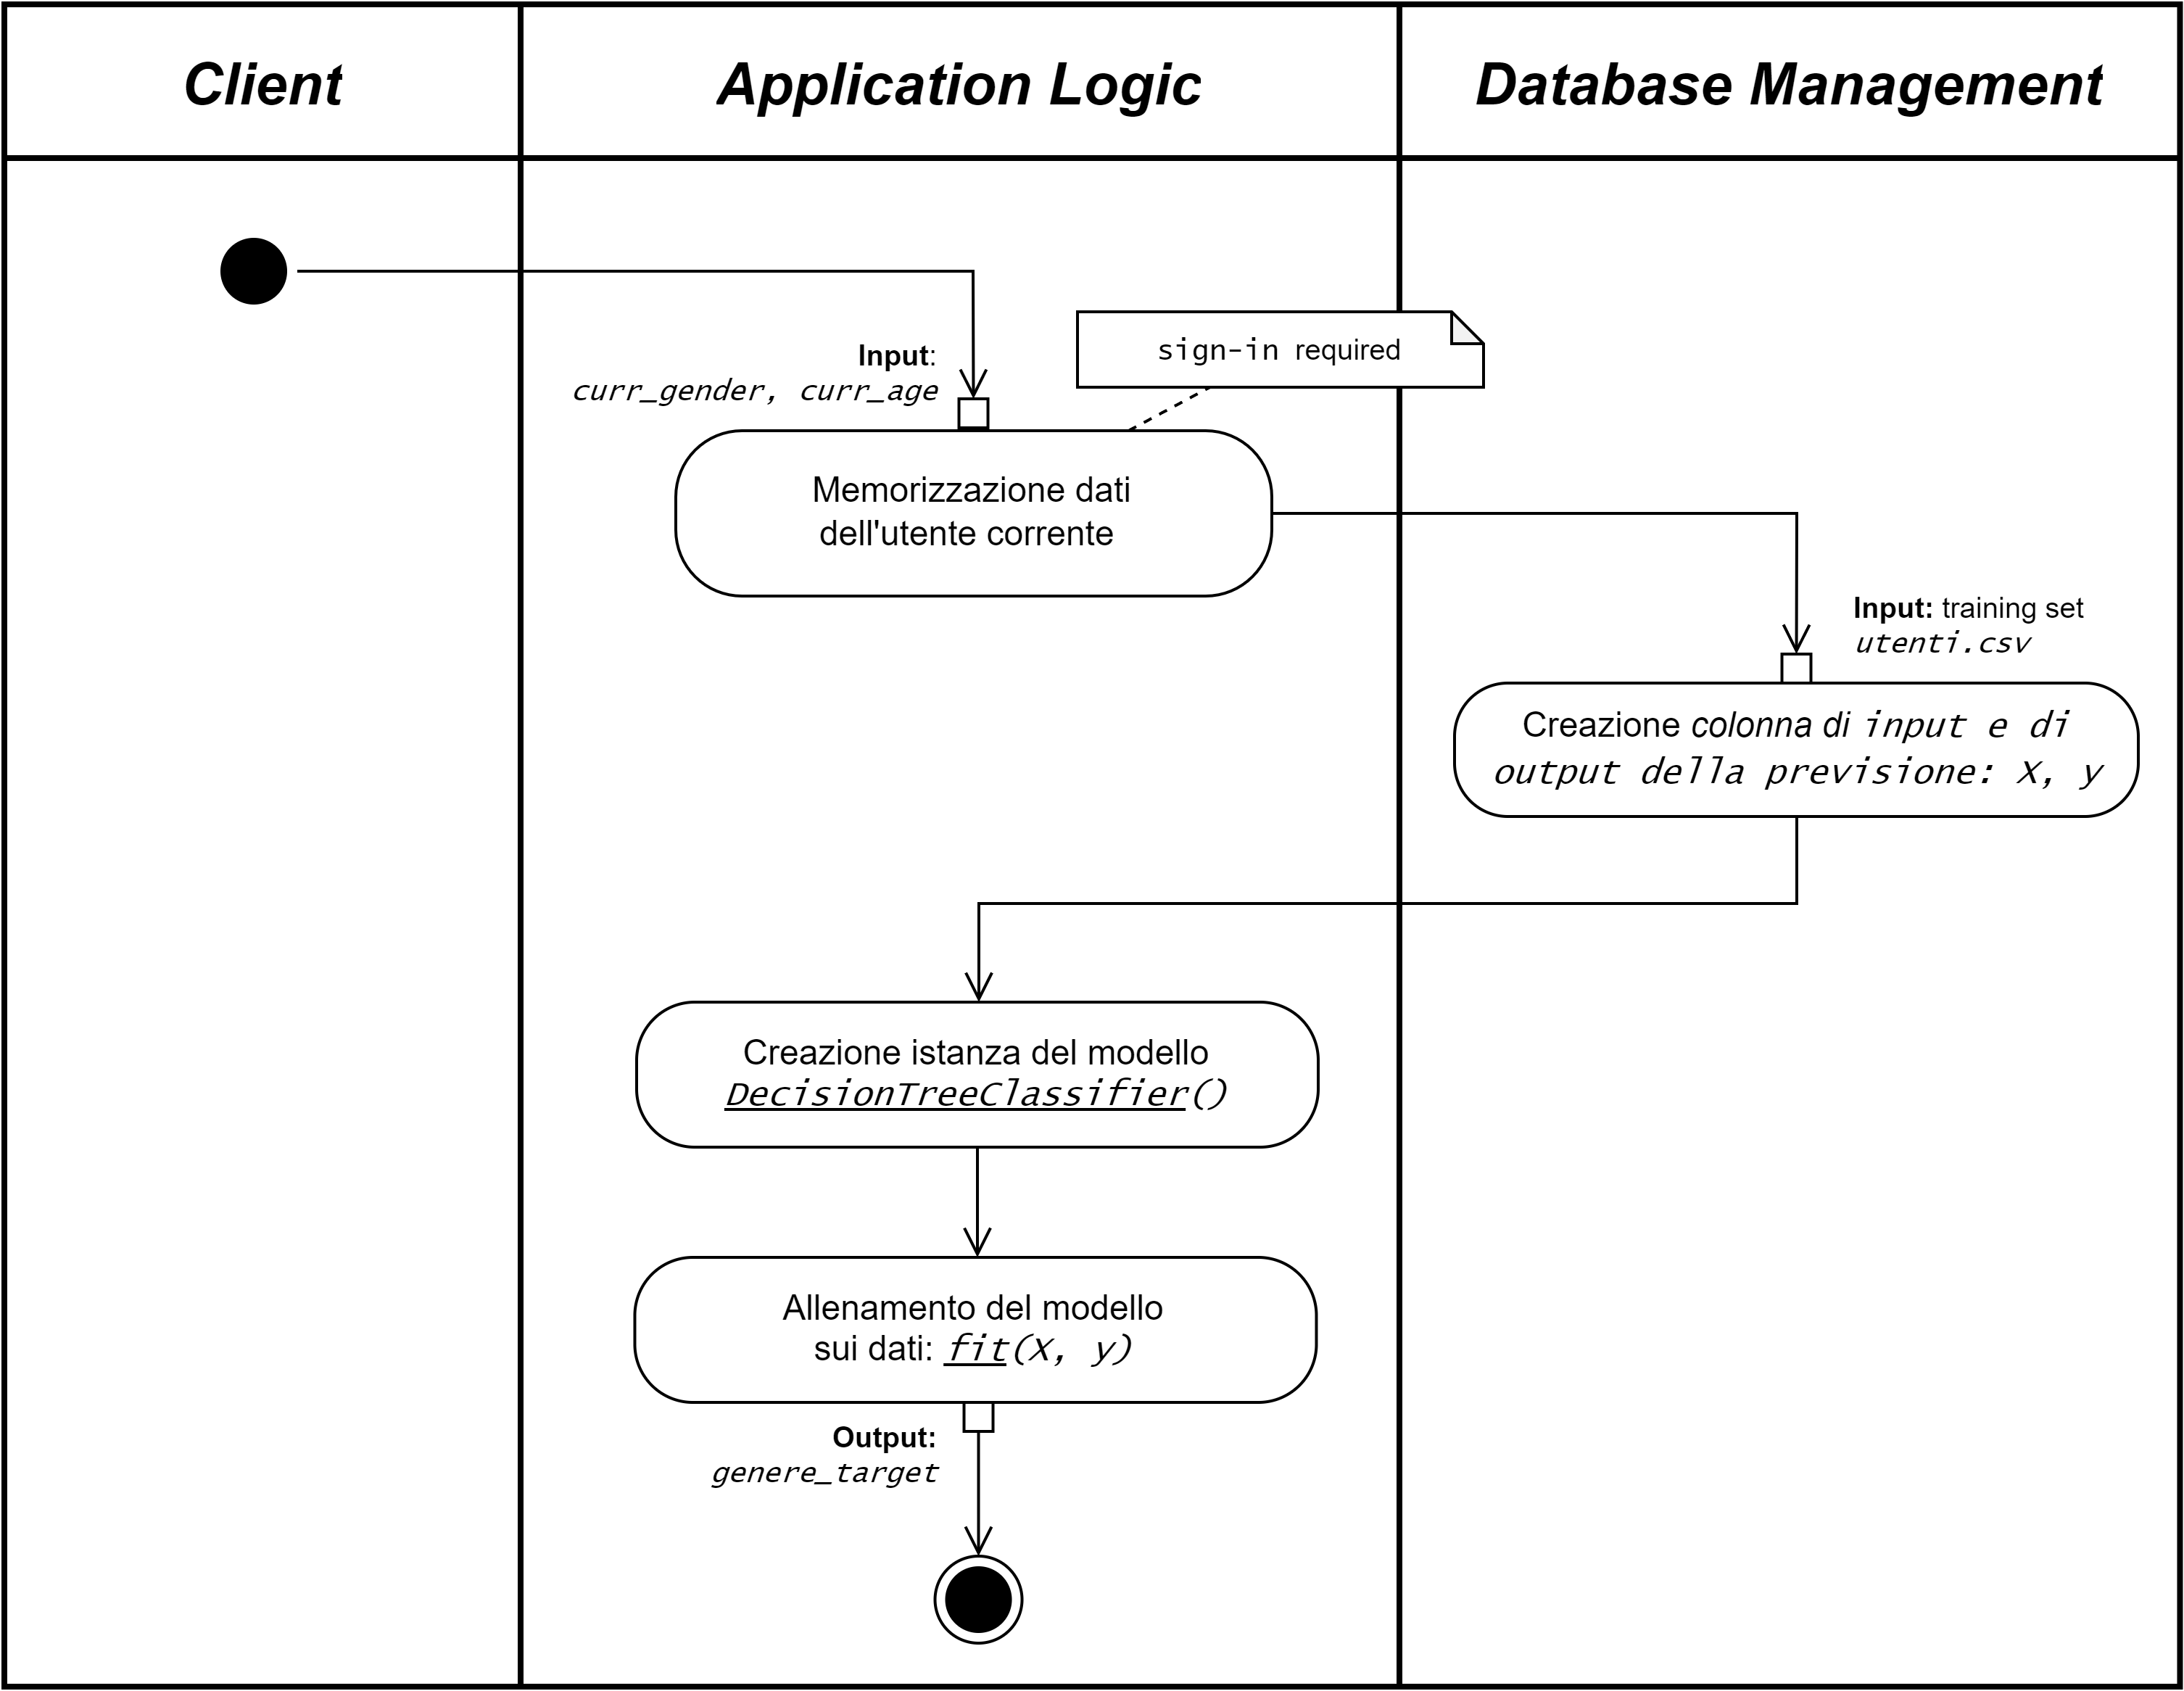
\includegraphics[scale=1]{images/flowchart_1_UML_ver2.png}
    \caption{UML Activity Diagram (parte I)}
    \label{fig-uml-ac-1}
\end{figure}


\newpage
\subsection{Algortimo Parte II}
\subparagraph{Pseudocodice}
%codice parte 2
Pseudocodice della seconda parte dell'algoritmo, relativa al suggerimento 
dei brani in base al genere target.
%\begin{figure}[H]
%    \centering
%    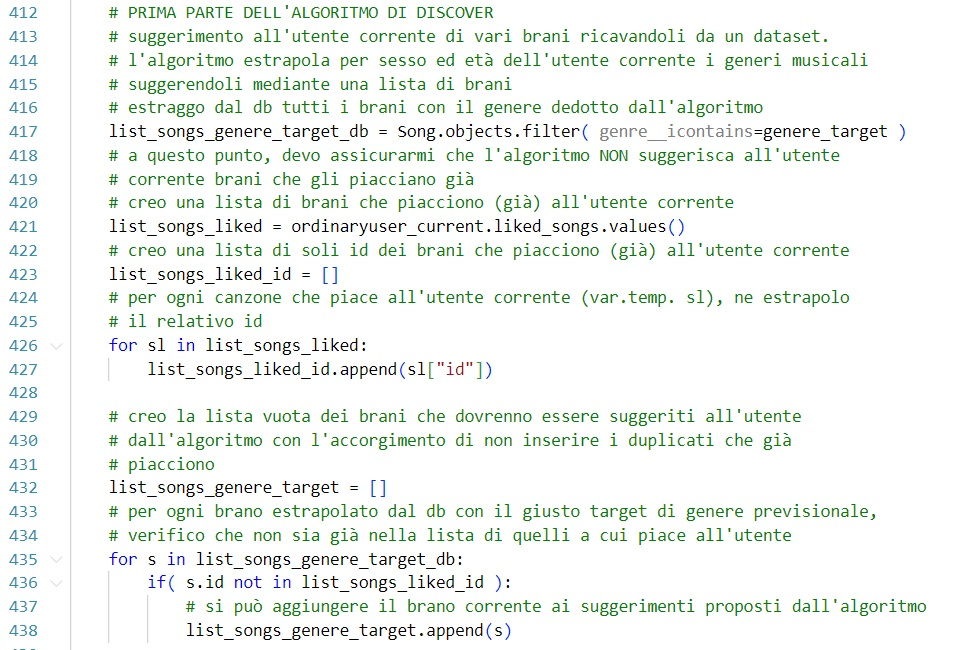
\includegraphics[scale=0.5]{images/alg2_v2.jpg}
%    \caption{Codice (parte II)}
%    \label{fig-codice2}
%\end{figure}
% pseudocodice 2
\begin{algorithm}
    \caption{Step 2 - Brani}
    \SetAlgoLined
    \SetKwProg{myalg}{algoritmo}{ begin}{end}
    \myalg{Discover($curr\_gender$, $curr\_age$)}{
        \BlankLine
        \textbf{...}
        \BlankLine
        \textbf{/* Estrazione dei brani con genere target */}\

        \textbf{do}{
            $songs\_list\_db \leftarrow Songs.\underline{filter}(genere=genere\_target)$
        }
        \BlankLine
        \BlankLine
        \textbf{/* Creazione lista dei brani che piacciono all'utente */}\

        \textbf{do}{
            $liked\_songs\_list \leftarrow curr\_user.liked\_song.\underline{values}()$
        }
        \BlankLine
        \BlankLine
        \textbf{/* Creazione lista vuota per gli id */}\

        \textbf{do}{
            $liked\_songs\_list\_id \leftarrow [] $
        }
        \BlankLine
        \BlankLine
        \textbf{/* Inserimento degli ID nella lista */}\

        \For{sl in liked\_songs\_list}{
            $liked\_songs\_list\_id.\underline{append}(sl[id])$
            
        }
        \BlankLine
        \BlankLine
        \textbf{/* Creazione lista per i brani da suggerire all'utente*/}\

        \textbf{do}{
            $songs\_list \leftarrow [] $
        }
        \BlankLine
        \BlankLine
        \textbf{/* Creazione lista vuota per i brani da suggerire all'utente*/}\

        \For{s in songs\_list\_db}{
            \If{s.id not in liked\_songs\_list\_id}{
                $songs\_list.\underline{append}(s)$
            }
        }
        \BlankLine
        \Return{$songs\_list$}\\
        \textbf{...}
        \BlankLine
        \KwResult{Lista brani con genere target}
        \BlankLine
        %\vspace{0.5cm}   
    }
\end{algorithm}
%flowchart 2
\newpage
%\subparagraph{Diagramma di flusso}
%Diagramma di flusso della seconda parte dell'algoritmo.
%\begin{figure} [H]
%    \centering
%    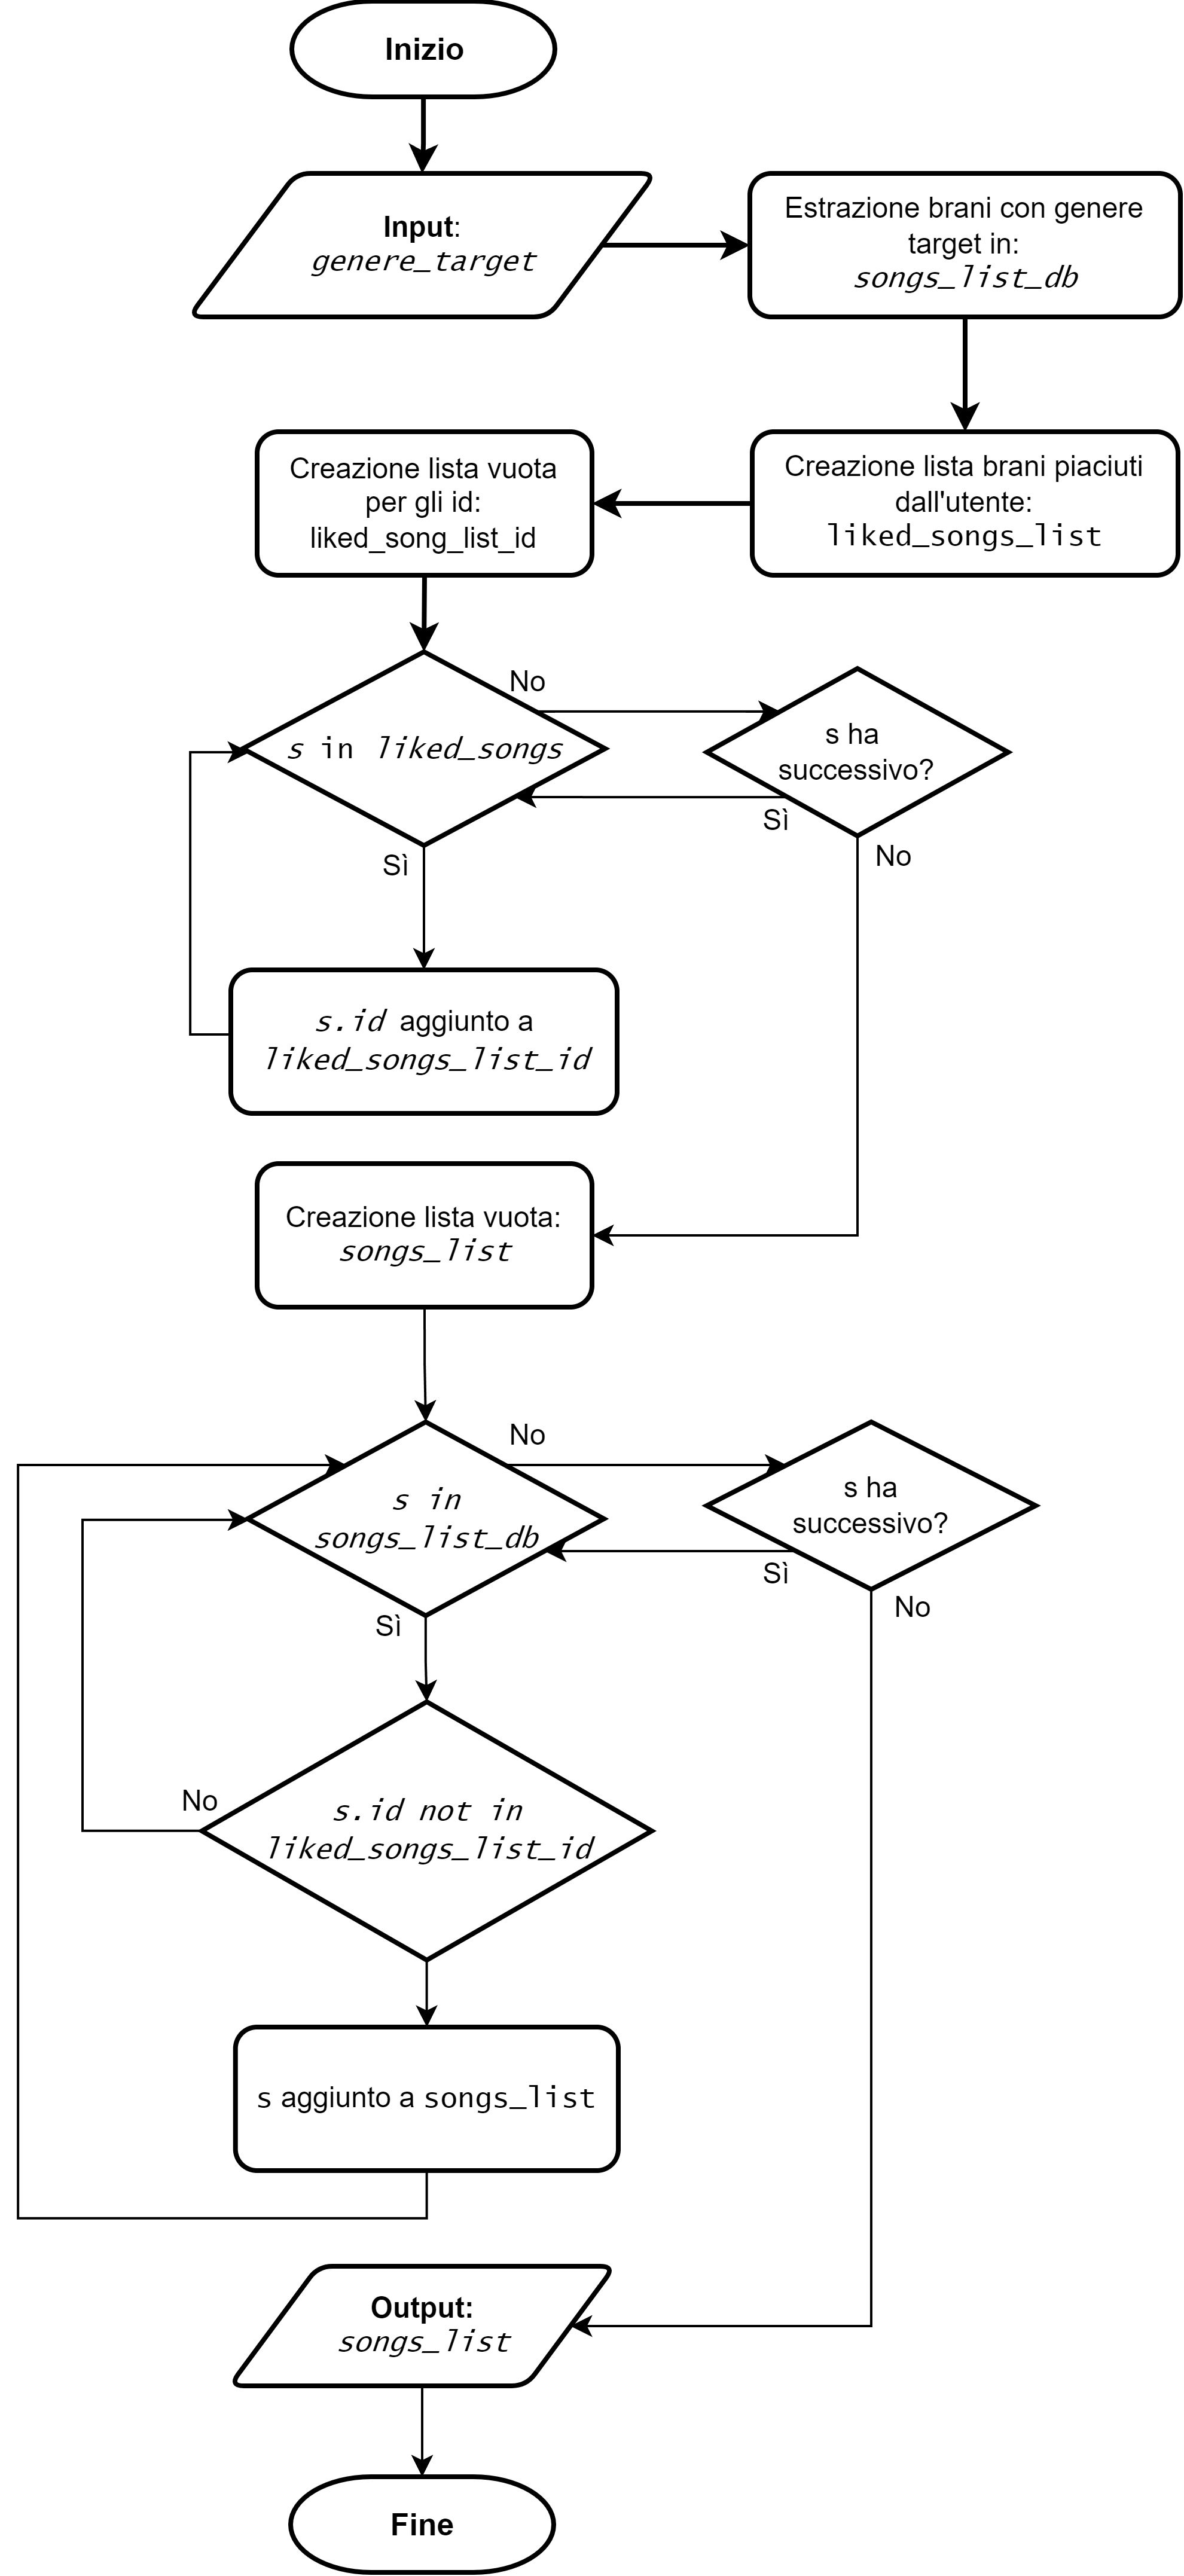
\includegraphics[scale=0.62]{images/flowchart-Parte II.png}
%    \caption{Flowchart (parte II)}
%    \label{fig-fc2}
%\end{figure}
\subparagraph{UML Activity Diagram}
Diagramma delle attività della seconda parte dell'algoritmo.
\begin{figure} [H]
    \centering
    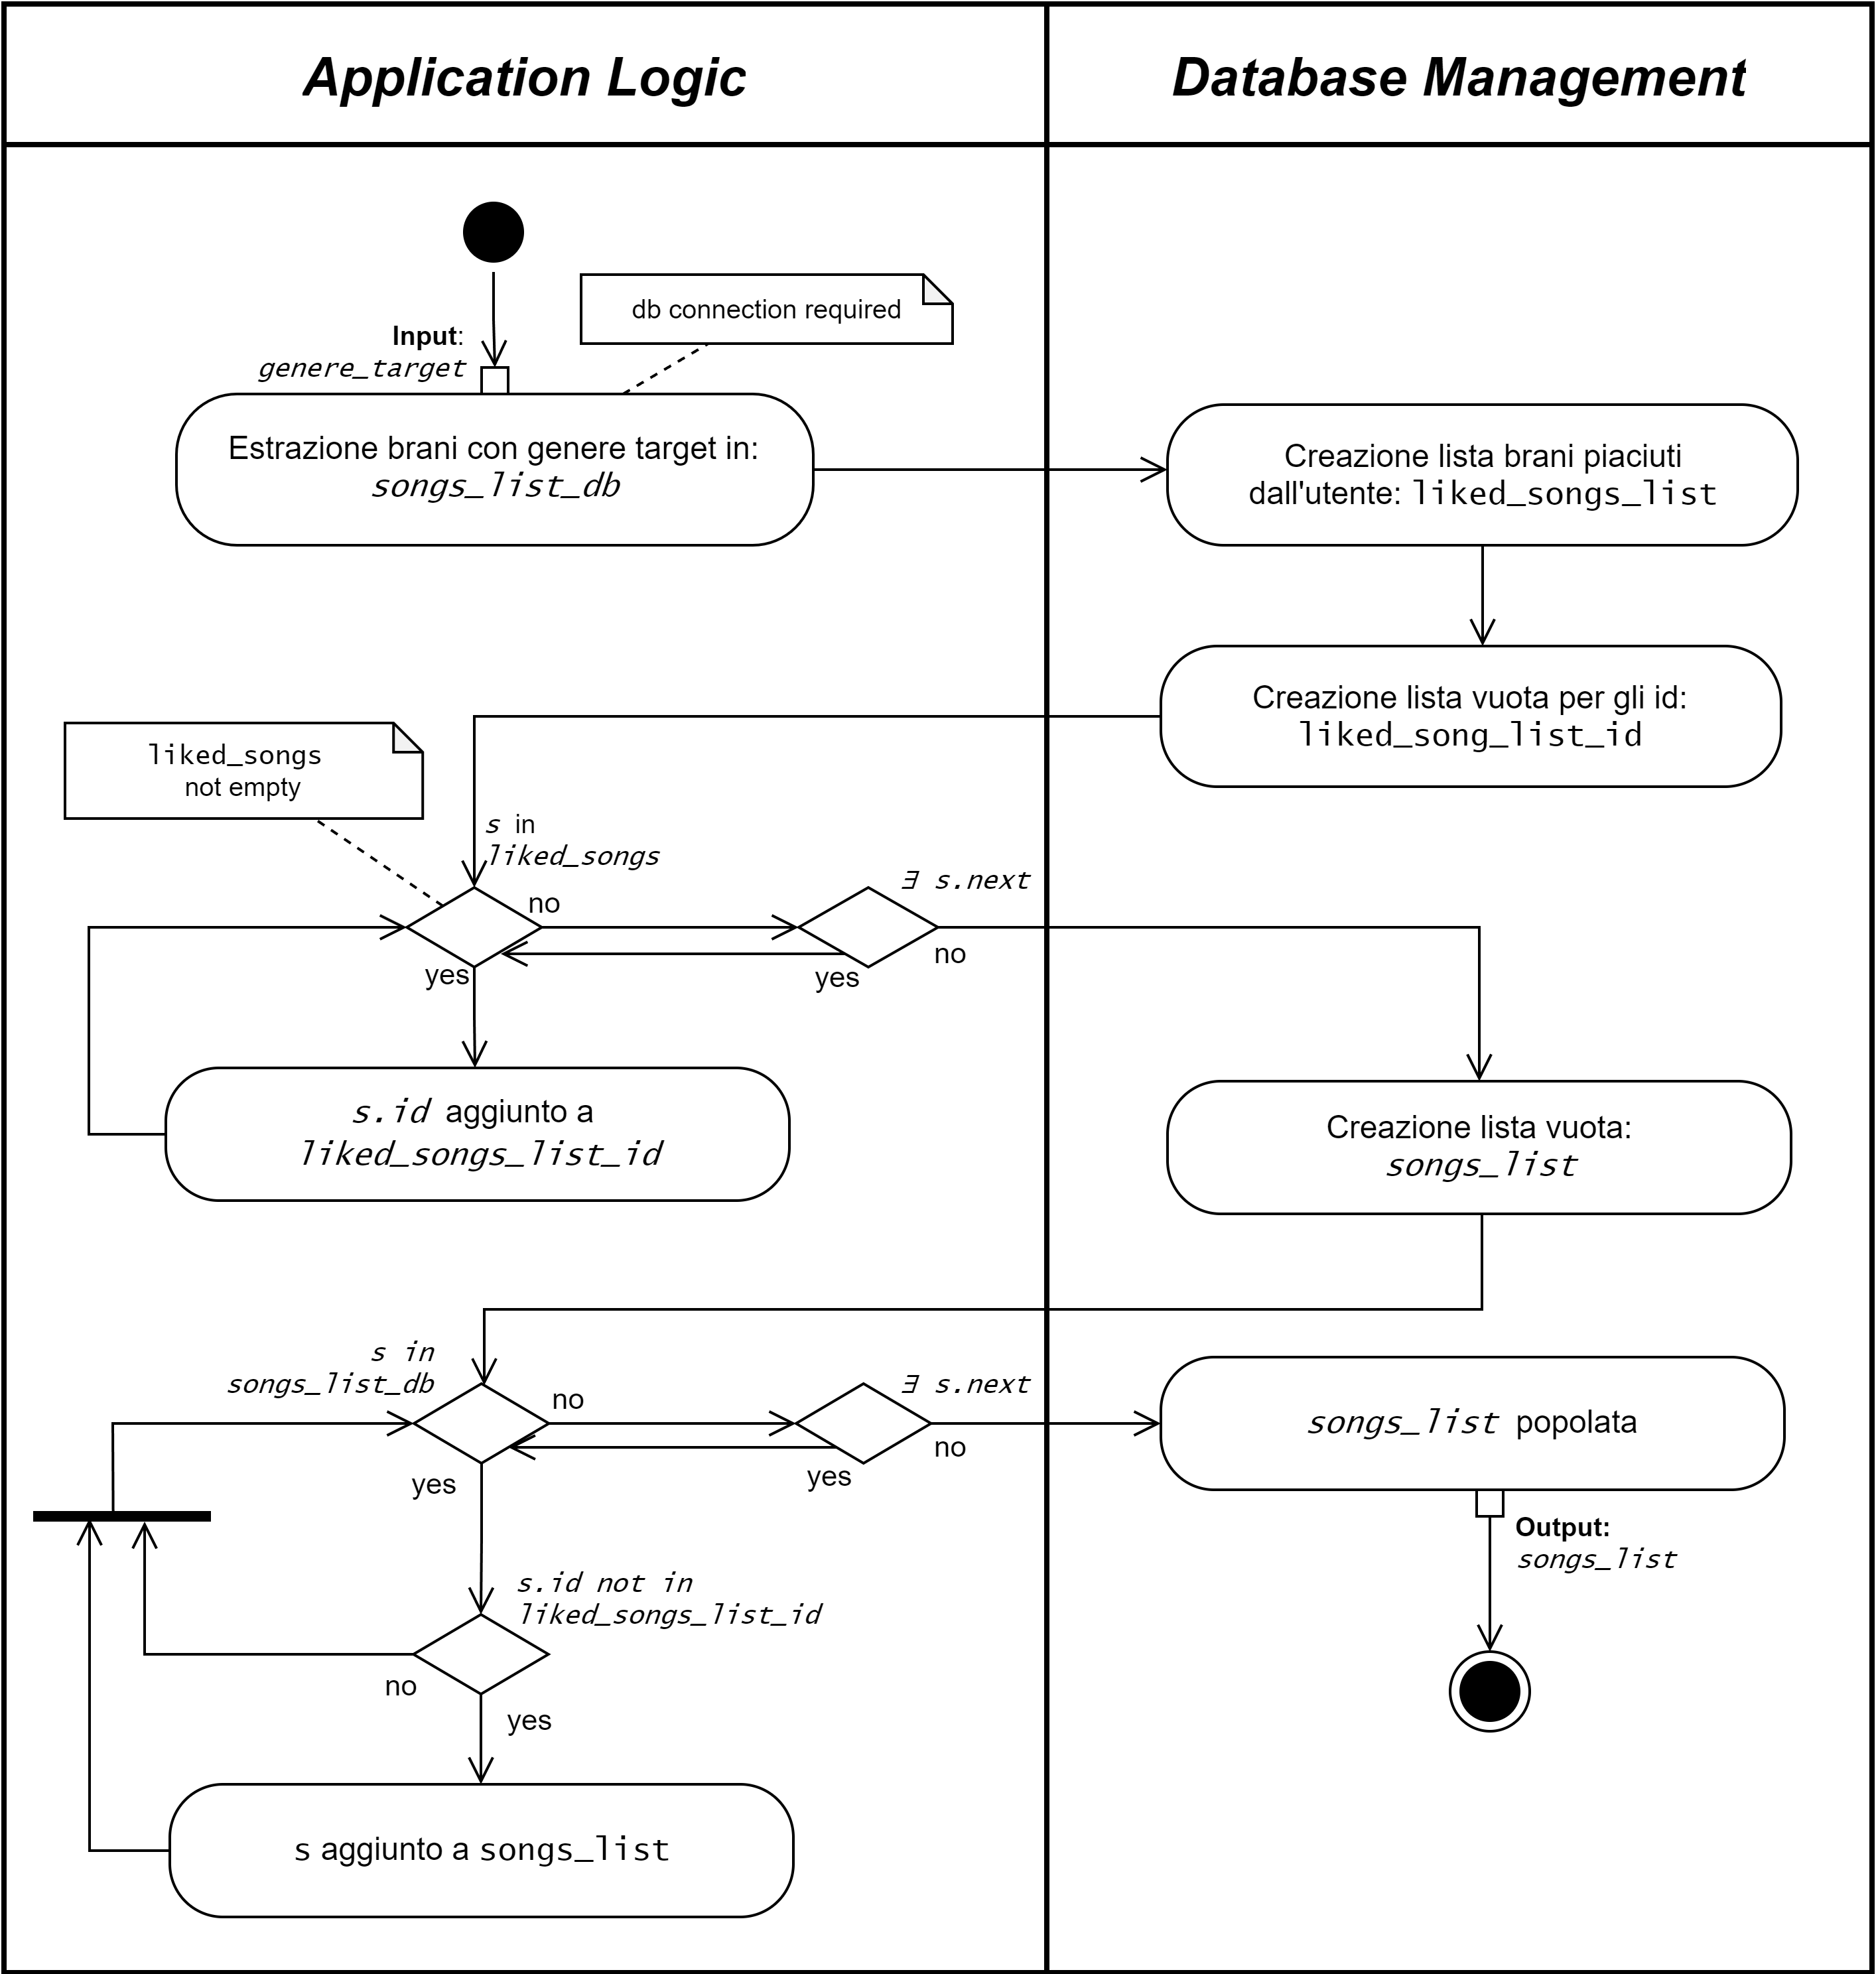
\includegraphics[scale=0.75]{images/flowchart_2_UML_ver2.png}
    \caption{UML Activity Diagram (parte II)}
    \label{fig-uml-ac-2}
\end{figure}




\newpage
\subsection{Algoritmo Parte III}

% codice 3
\subparagraph{Pseudocodice}
Pseudocodice della terza parte dell'algoritmo, quella relativa al
suggerimento di utenti con gusti simili. 
%\begin{figure}[H]
%    \centering
%    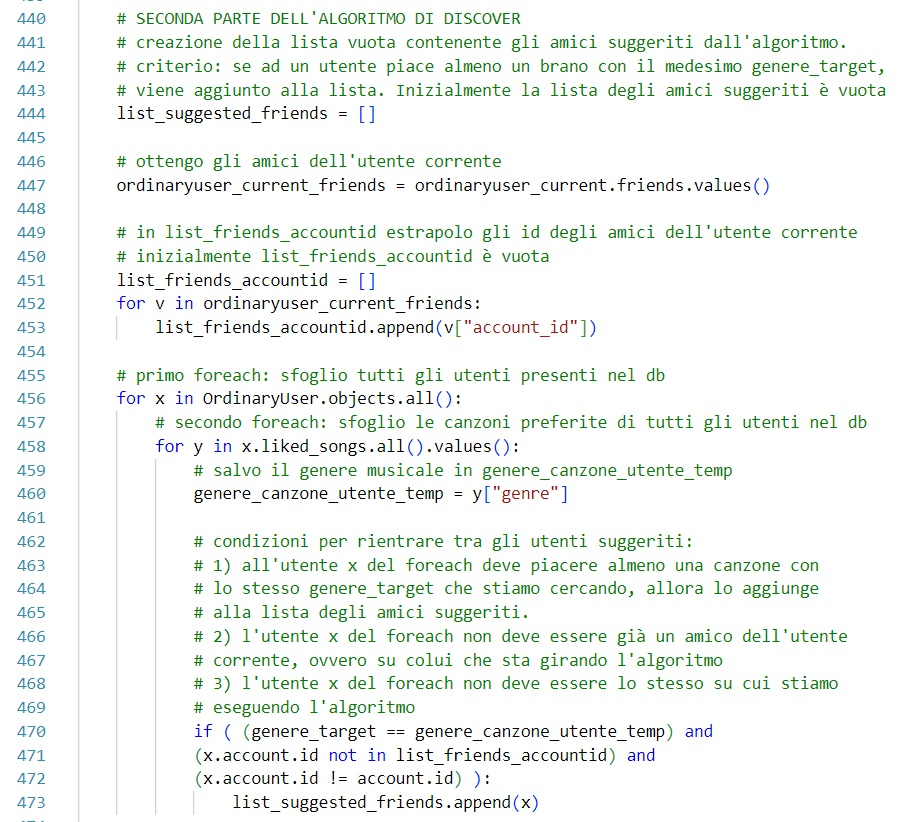
\includegraphics[scale=0.7]{images/alg3_v2.jpg}
%%    \caption{Codice (Parte III)}
%    \label{fig-codice3}
%\end{figure}


% pseudocodice 3
\begin{algorithm}
    \caption{Step 3 - Amici}
    \SetAlgoLined
       \SetKwProg{myalg}{algoritmo}{ begin}{end}
    \myalg{Discover($curr\_gender$, $curr\_age$)}{
        \BlankLine
        \textbf{...}
        \BlankLine
        \textbf{/* Creazione lista vuota */}\\
        \textbf{do}{
            $[] \leftarrow list\_suggested\_friends $
        }

        \BlankLine
        \BlankLine
        \textbf{/* Memorizzazione della lista di amici dell'utente*/}\\
        \textbf{do}{
            $friends\_id \leftarrow curr\_user.friends.\underline{values}() $
        }

        \BlankLine
        \BlankLine
        \textbf{/* Creazione lista vuota */}\\
        \textbf{do}{
            $[ ] \leftarrow list\_user\_friends $
        }


        \BlankLine
        \BlankLine
        \For{v in friends\_id }{
            %\tcp{Blocco di istruzioni da eseguire per ogni valore di i}
            $list\_user\_friends.\underline{append}(v[id])$
            
        }
        \BlankLine
        \textbf{/* Memorizzazione amici dell'utente corrente */}\\
        \ForEach{ x in user.\underline{all}()}{
            \ForEach{y in x.liked\_songs.\underline{all}().\underline{values}()}{
                $genere\_temp \leftarrow y [genere] $\\
                \If{genere\_target = genere\_temp AND x.account.id != account.id AND x.account.id not in list\_user\_friends }{
                    list\_suggested\_friends.\underline{append}(x)
                }
            }
        }
    \BlankLine
    \Return{list\_suggested\_friends}\\
    \textbf{...}
    \BlankLine
    \KwResult{Lista utenti con gusti affini all'utente}
    \BlankLine
    }
\end{algorithm}

% flowchart 3
\newpage
%\subparagraph{Diagramma di flusso} 
%Diagramma di flusso della terza parte dell'algoritmo.
%\begin{figure} [H]
%    \centering
%    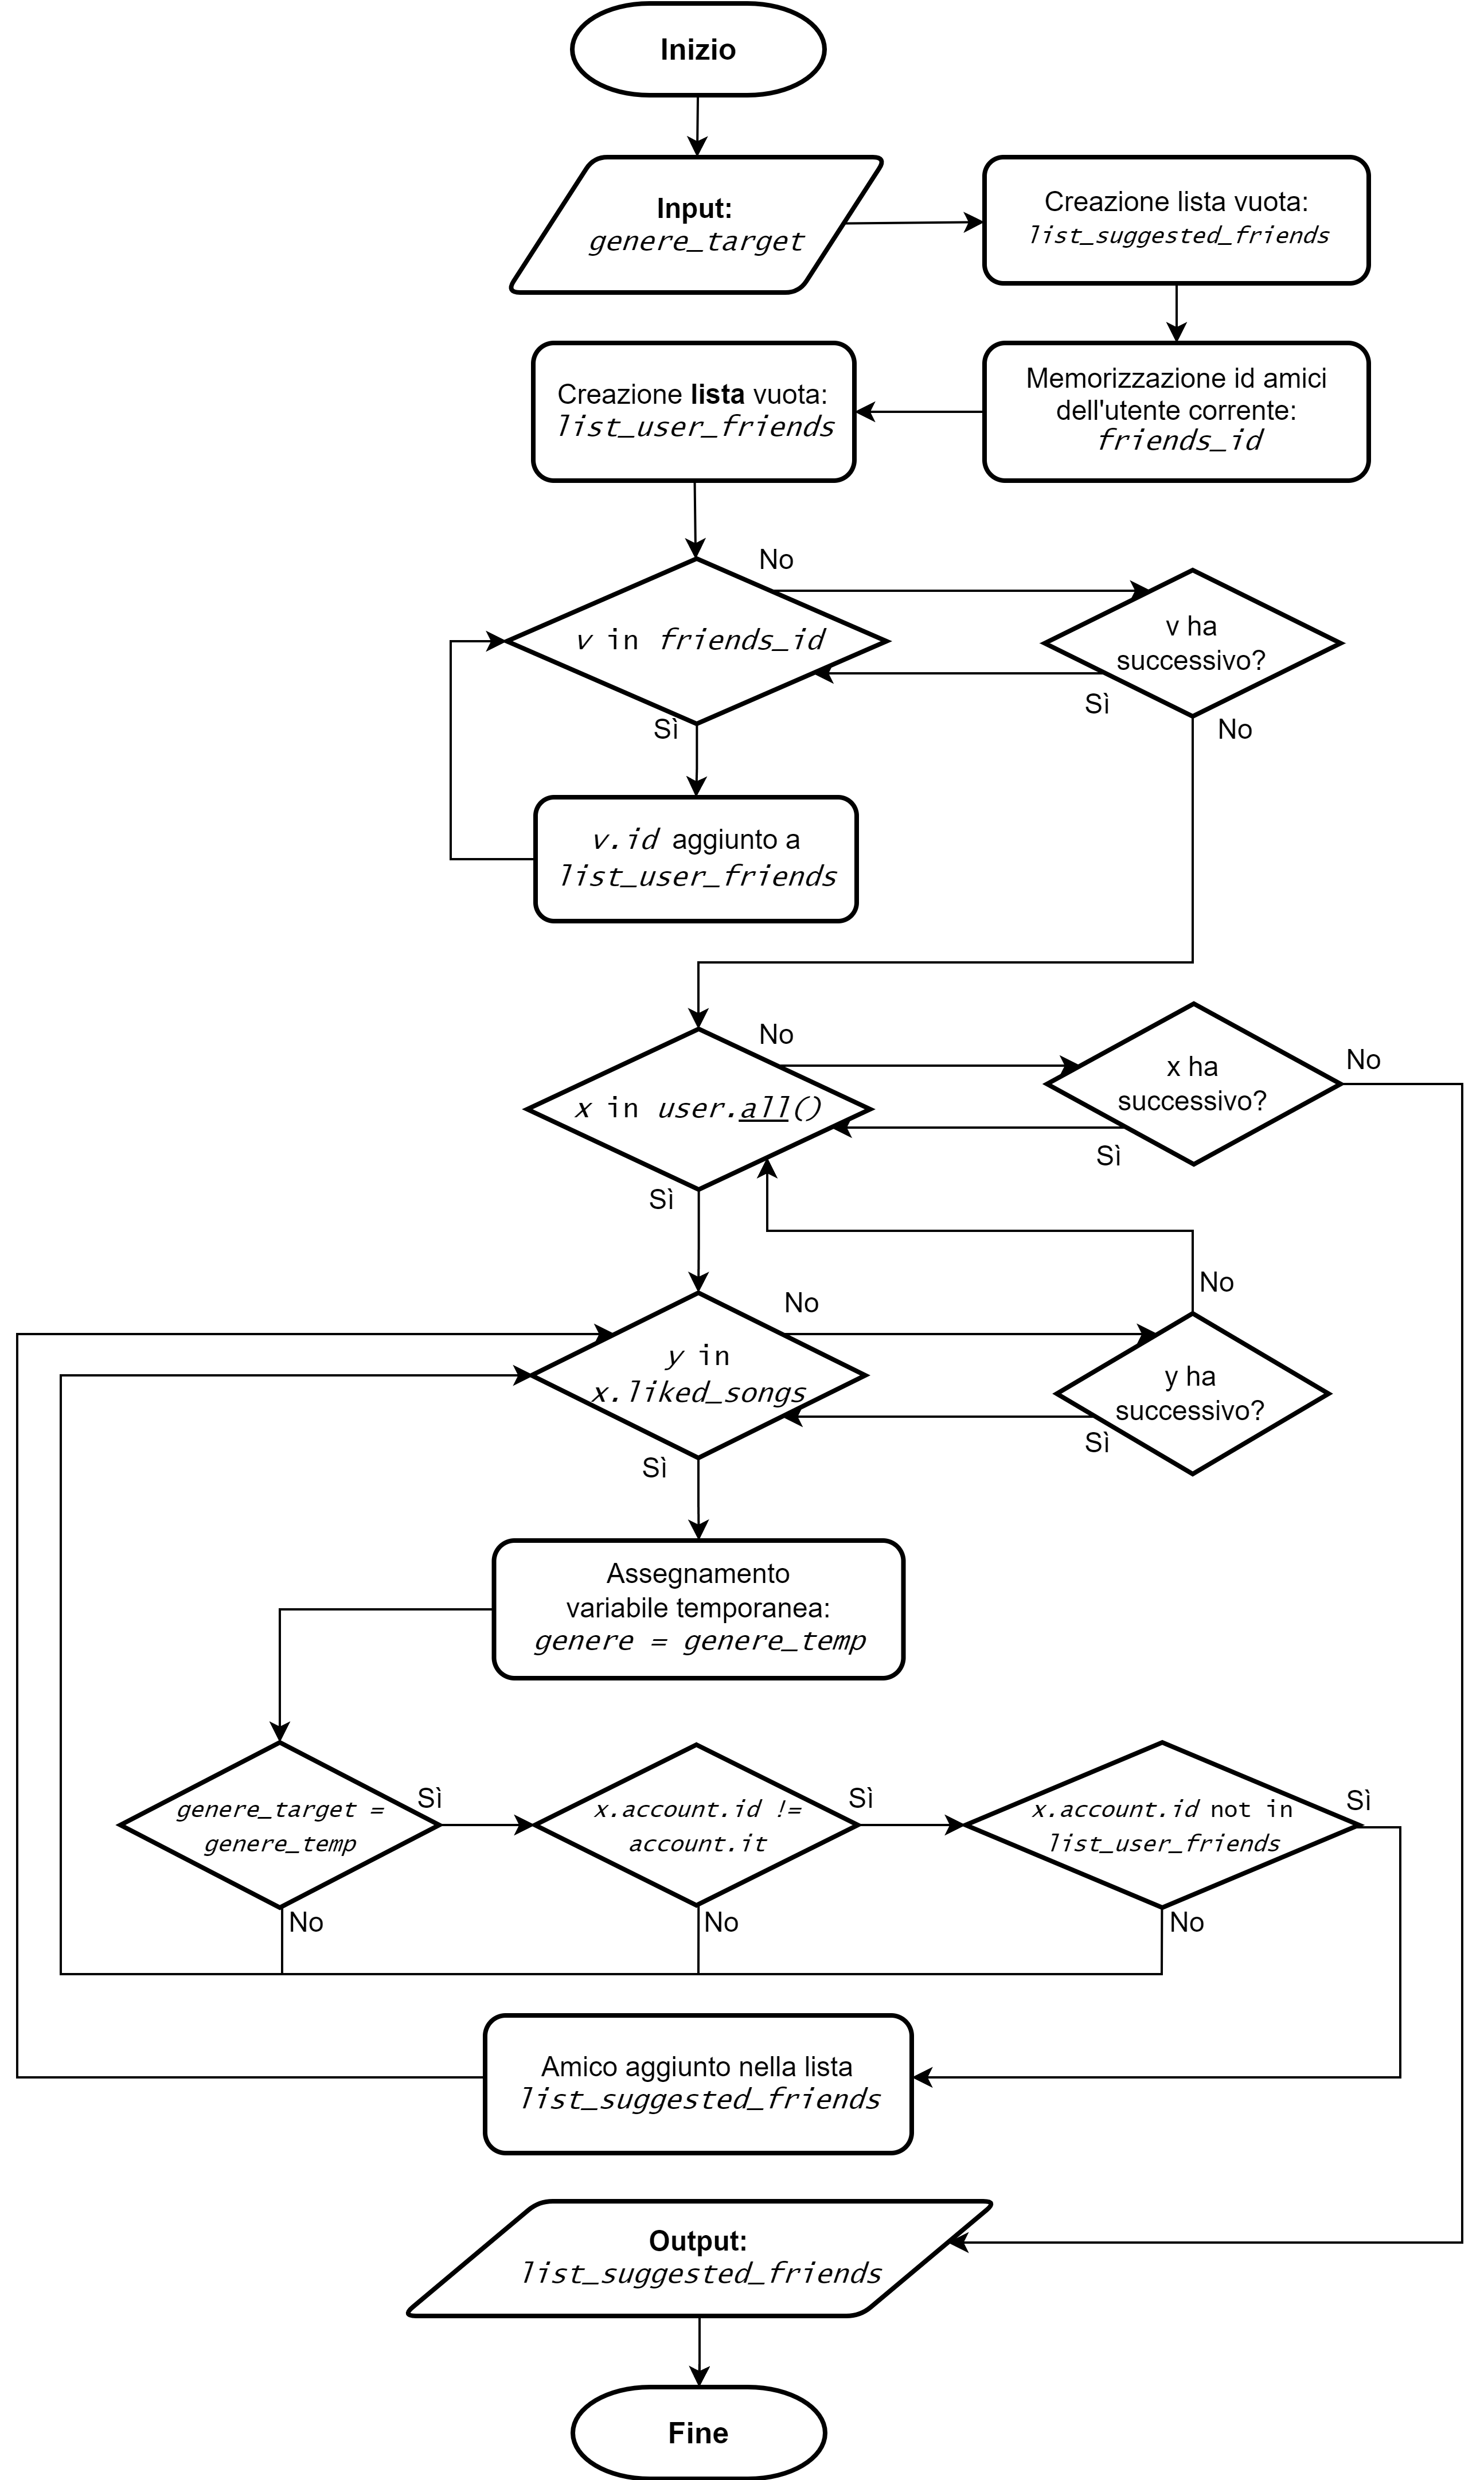
\includegraphics[scale=0.65]{images/flowchart-Parte III.png}
%    \caption{Flowchart (parte III)}
%    \label{fig-fc3}
%\end{figure}

\subparagraph{UML Activity Diagram}
Diagramma delle attività della terza parte dell'algoritmo.
\begin{figure} [H]
    \centering
    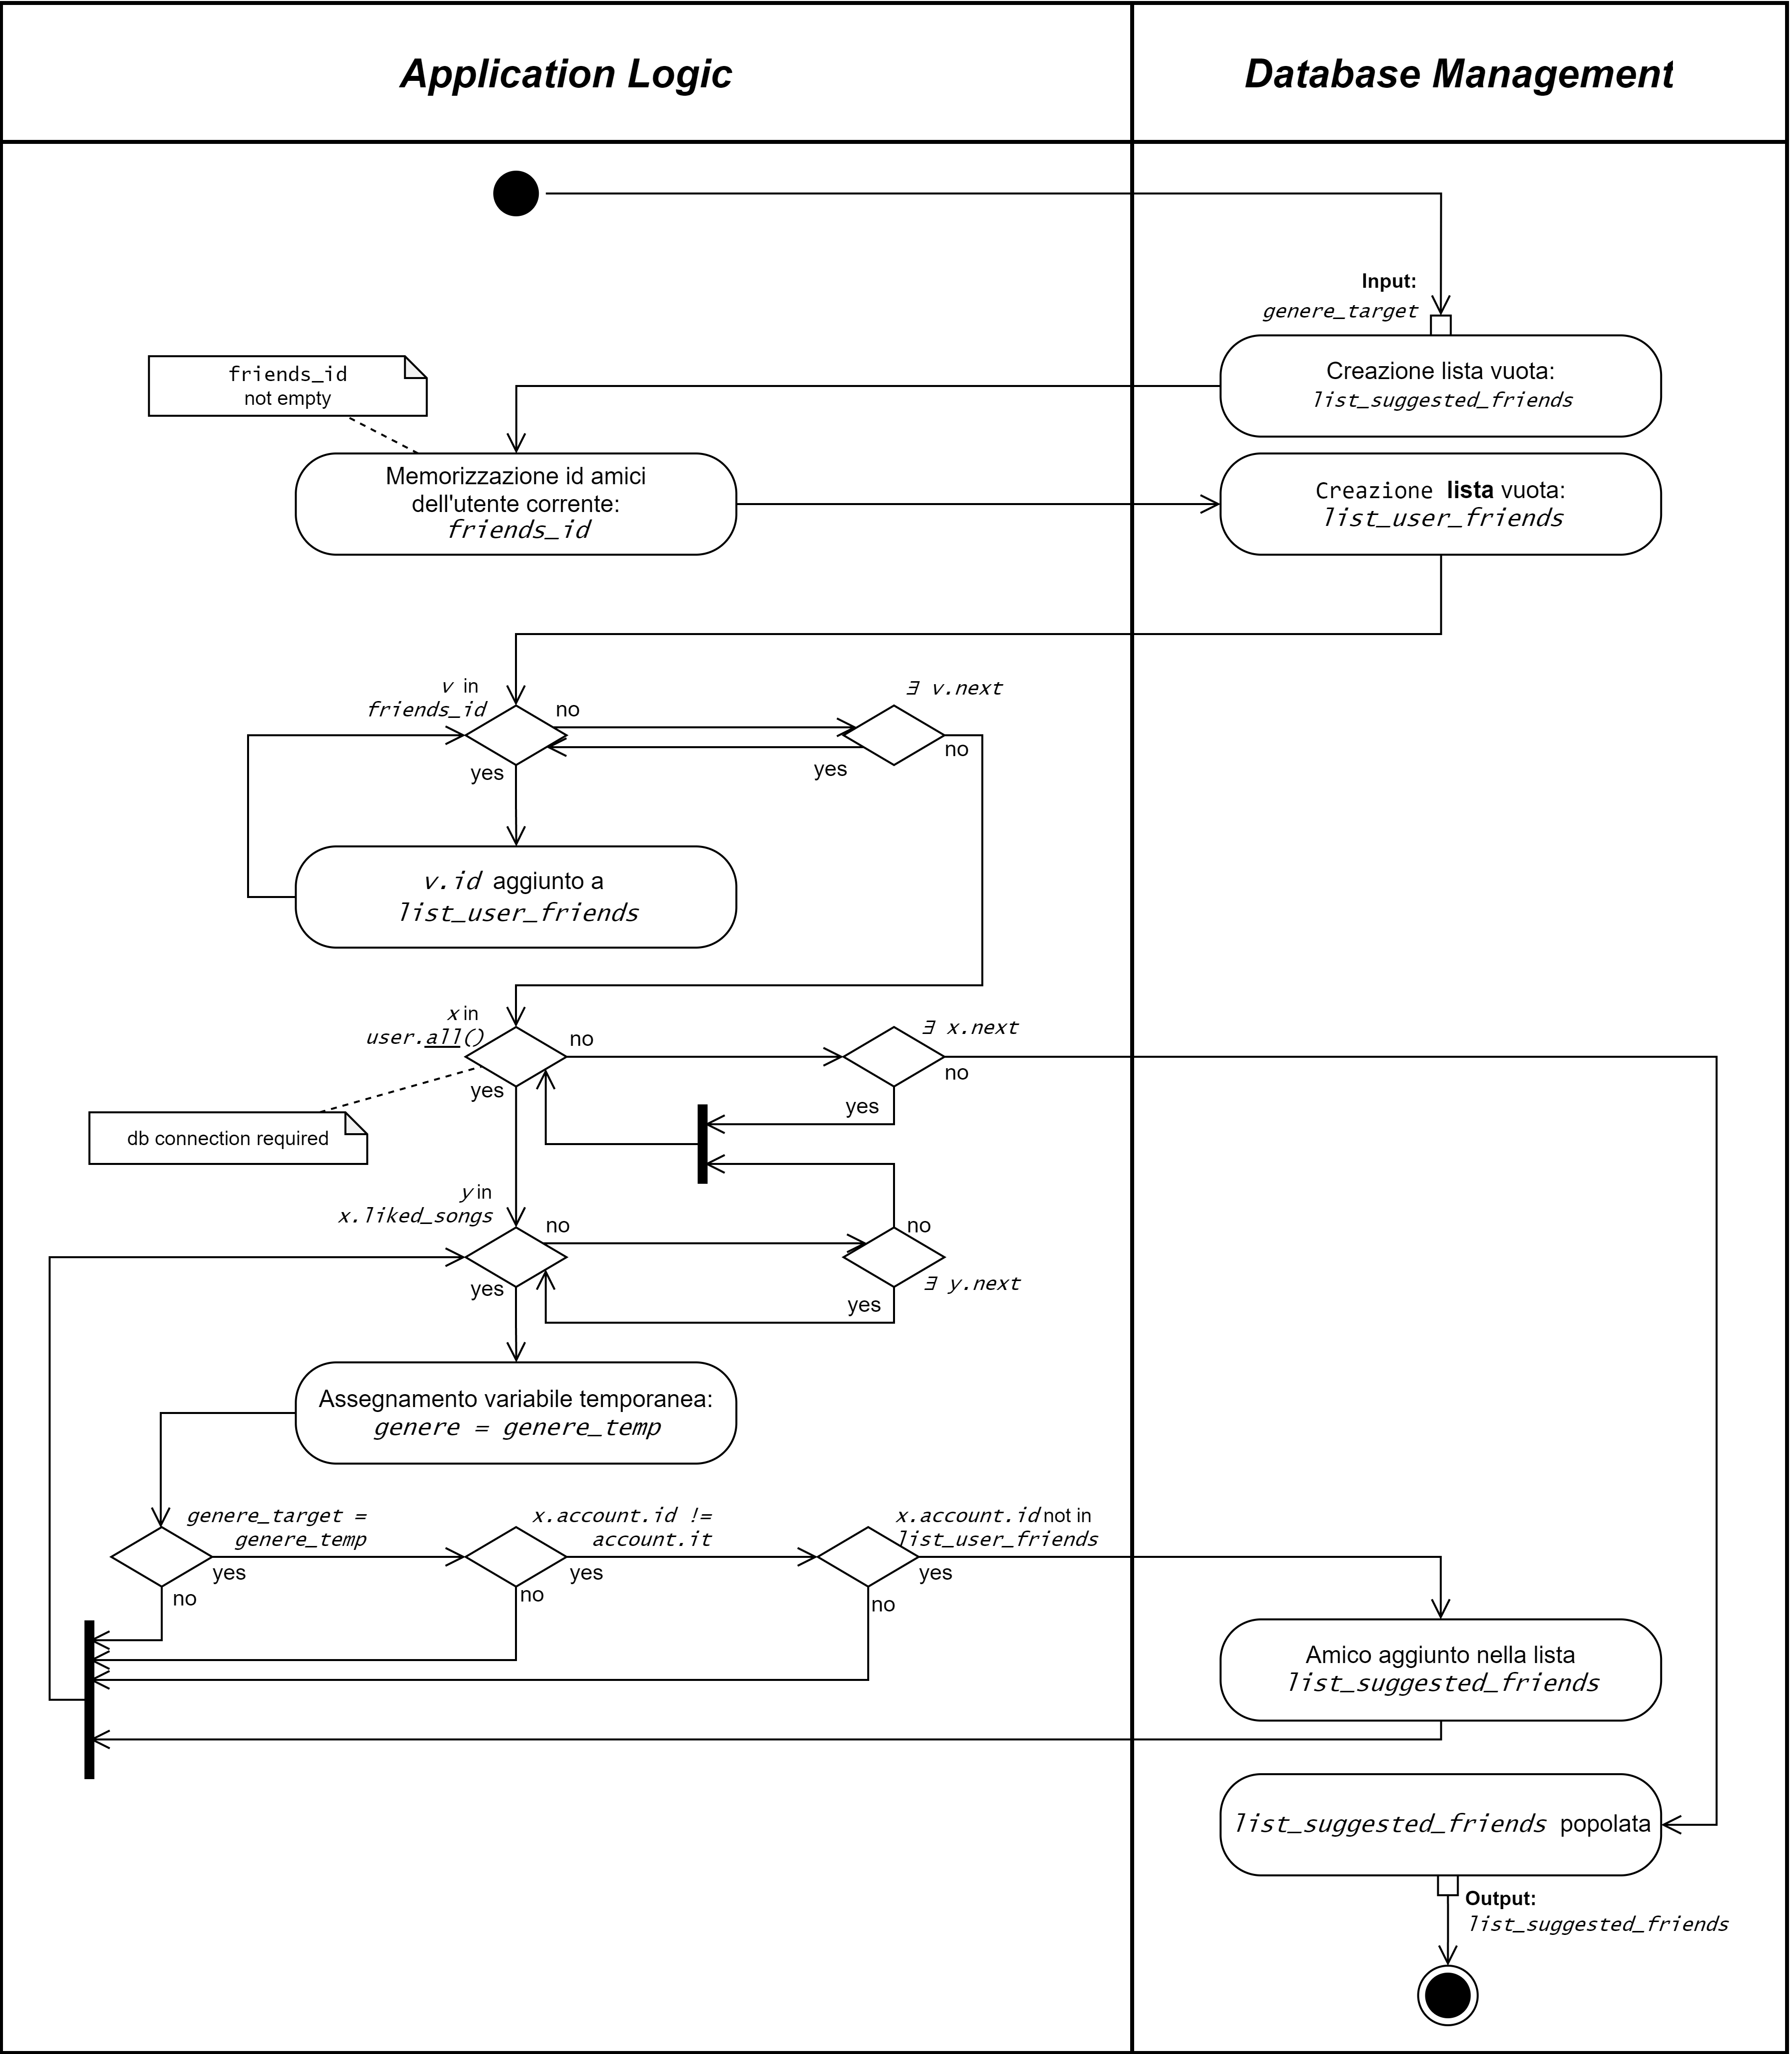
\includegraphics[scale=0.7]{images/flowchart_3_UML_ver2.png}
    \caption{UML Activity Diagram (parte III)}
    \label{fig-uml-ac-3}
\end{figure}



\newpage
\subsection{Algoritmo Parte IV}
% codice 4

\subparagraph{Pseudocodice}
Pseudocodice dell'ultima parte dell'algoritmo.  
%\begin{figure}[H]
%    \centering
%    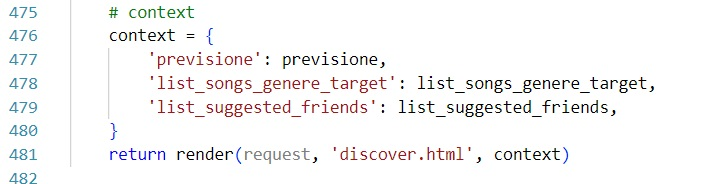
\includegraphics[scale=0.7]{images/alg4_v2.jpg}
%    \caption{Codice (parte IV)}
%    \label{fig-codice4}
%\end{figure}
%\vspace{0.5cm}

% pseudocodice 4
\begin{algorithm}

    \caption{Step 4 - Parametri di ritordno}
    \SetAlgoLined
   
    \SetKwProg{myalg}{algoritmo}{ begin}{end}
    \myalg{Discover($curr\_gender$, $curr\_age$)}{
        \BlankLine
        \BlankLine
        \textbf{...}
        \BlankLine
        \BlankLine
        \textbf{/* Ritorno parametri di interesse */}\\
        \Return{songs\_list}\\
        \Return{list\_suggested\_friends}\\    
        \BlankLine
        \BlankLine
        \KwResult{Lista brani con genere target e lista utenti con gusti affini all'utente }
        \vspace{0.5cm}
        %\label(alg:1)
    }
\end{algorithm}
% flowchart 4
\vspace{1cm}
%\subparagraph{Diagramma di flusso} Diagramma di flusso dell'ultima parte dell'algoritmo.
%\begin{figure} [H]
%    \centering
%    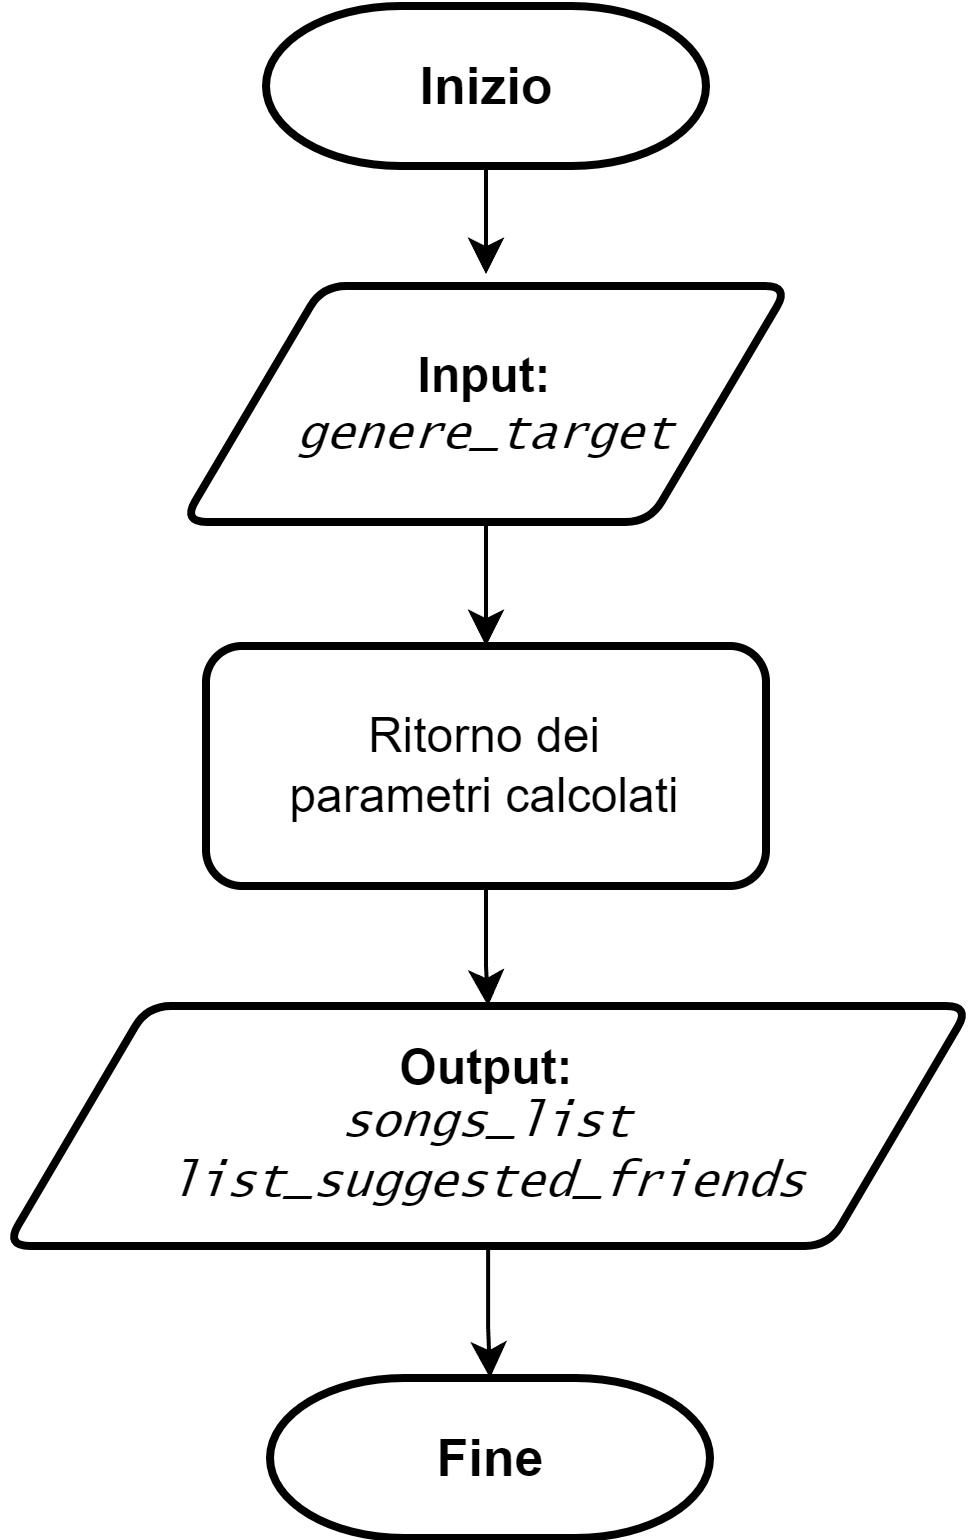
\includegraphics[scale=0.7]{images/flowchart-Parte IV.png}
%    \caption{Flowchart (parte IV)}
%    \label{fig-fc4}
%\end{figure}
\subparagraph{UML Activity Diagram}
Diagramma delle attività della parte finale dell'algoritmo.
\vspace{0.3cm}
\begin{figure} [H]
    \centering
    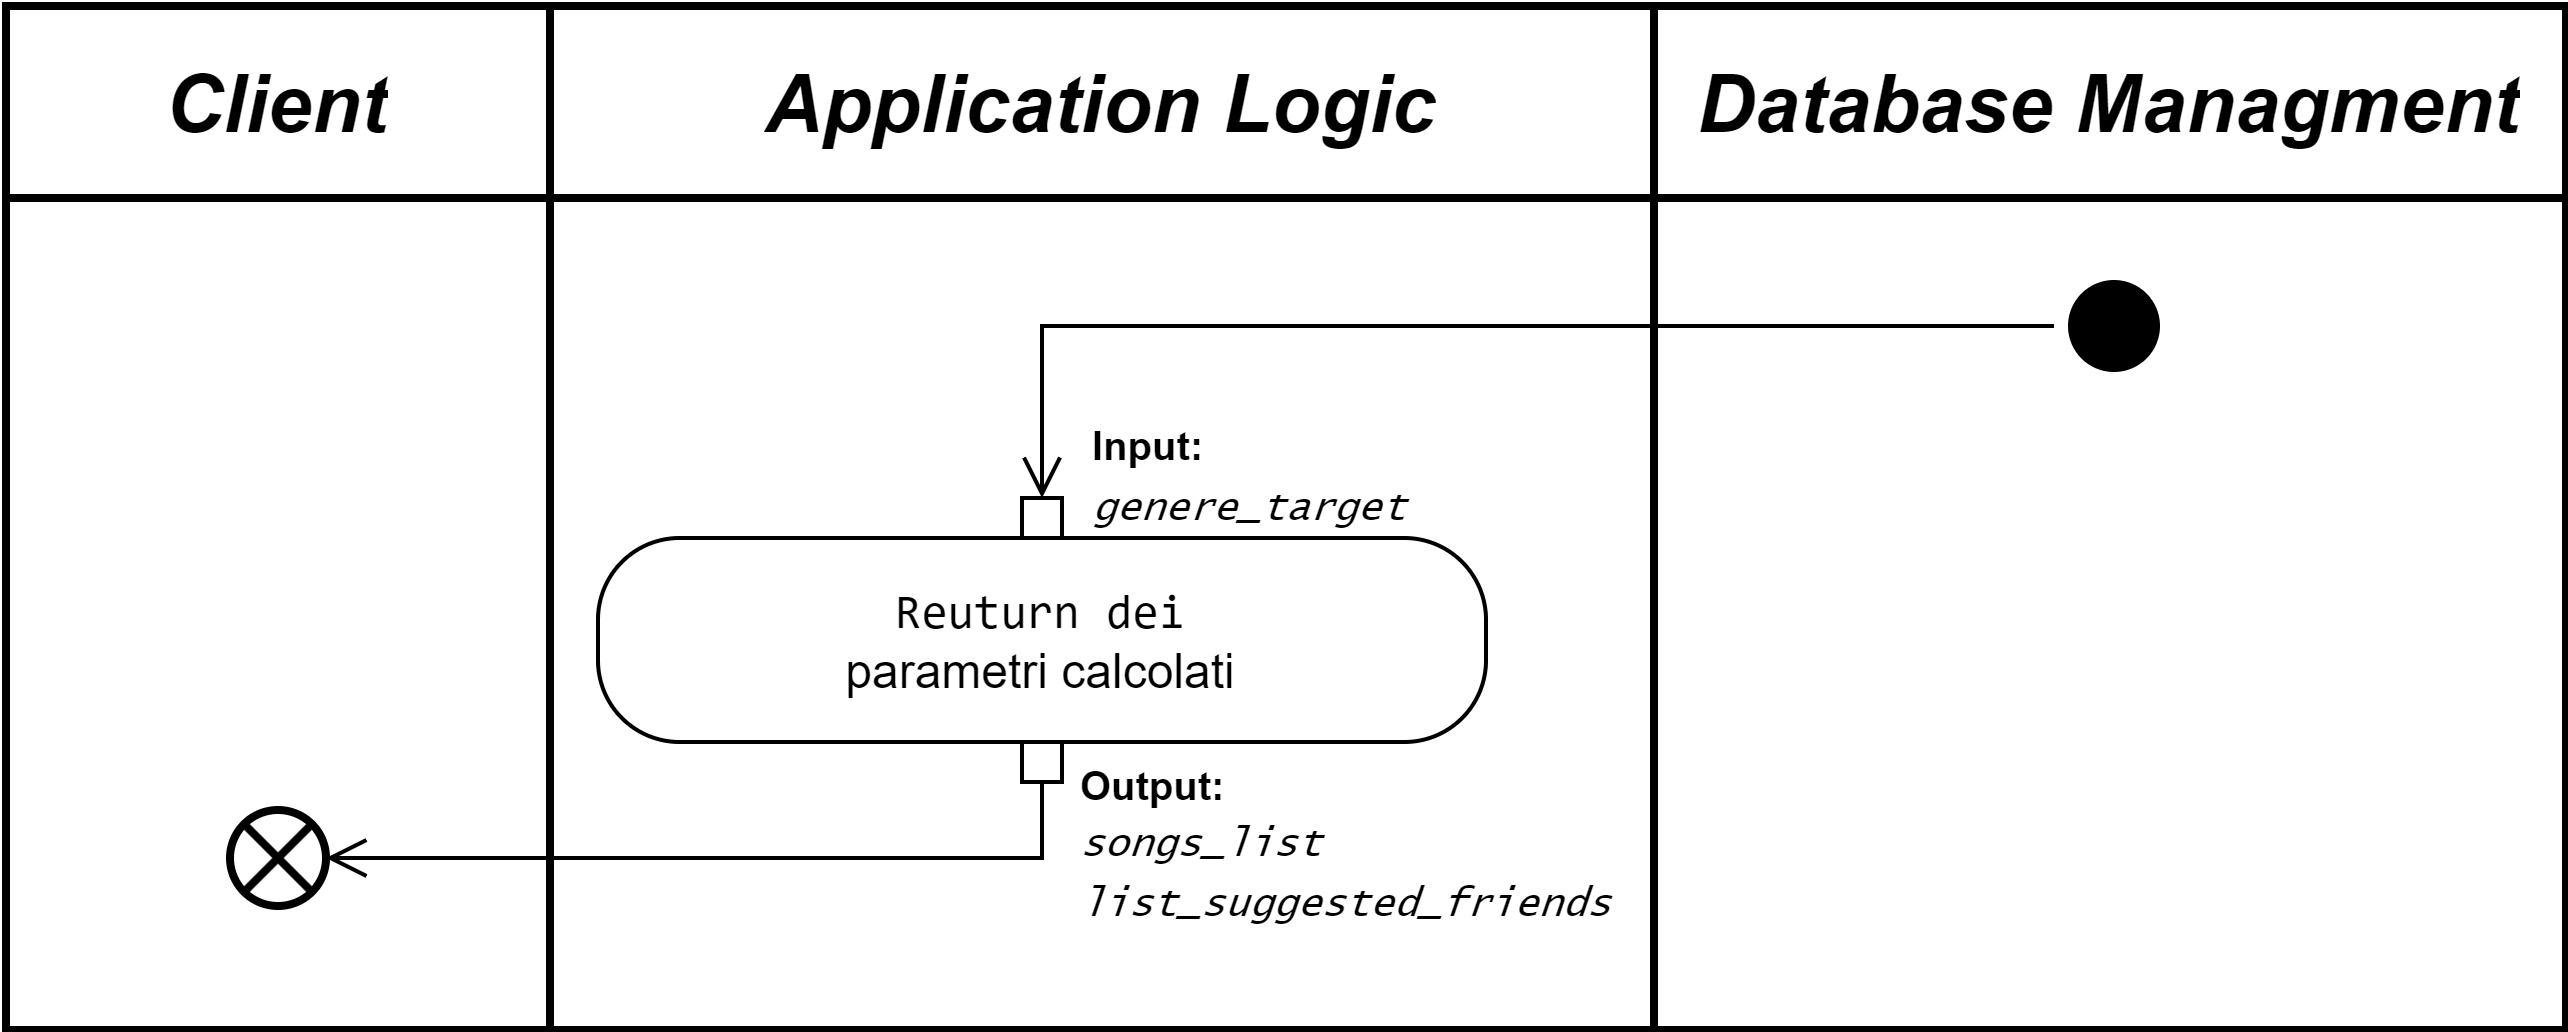
\includegraphics[scale=0.8]{images/flowchart_4_UML_ver2.png}
    \caption{UML Activity Diagram (parte IV)}
    \label{fig-uml-ac-4}
\end{figure}




\newpage
\subsection{Analisi della complessità}
Per valutare la complessità temporale dell'algoritmo, vengono esaminate le operazioni principali che 
vengono eseguite e e viene analizzato come queste operazioni dipendono dalla dimensione dell'input. 
Di seguito viene fornita una stima approssimativa della complessità temporale per ogni parte dell'algoritmo:

\begin{itemize}
    \item \textbf{Lettura del file CSV:} La lettura del file CSV tramite la funzione $read\_csv$ ha una 
    complessità temporale che dipende dalla dimensione del file, nello specifico dal numero di righe e colonne del file.
    Supponiamo che ci siano n righe e m colonne nel file. La lettura del file richiede un'operazione 
    per ogni cella nel file, di conseguenza la complessità è dell'ordine di ${O(n*m)}$.
    % sono 21 righe e 3 colonne, quindi può essere considerata costante O(1)
    \item \textbf{Creazione e addestramento del modello di classificazione:} La creazione del modello 
    \textit{DecisionTreeClassifier} e l'addestramento del modello tramite il metodo \textit{fit} dipendono dal numero di 
    caratteristiche e dal numero di esempi nel set di dati. Se denotiamo con p il numero di istanze (quindi n, le righe del file csv) 
    e con q il numero di attributi (m, il numero di colonne), allora la complessità temporale può essere approssimata a $O(p * q log(p))$, 
    poiché la costruzione di un albero decisionale richiede operazioni che dipendono da entrambi i valori.
    % sono 21 istanze e 3 colonne, quindi può essere approssimato a O(1) costante
    \item \textbf{Previsione dei generi musicali:} La previsione dei generi musicali per 
    l'utente corrente utilizzando il modello addestrato ha una complessità temporale di 
    $O(1)$, poiché si tratta di un singolo esempio (operazione costante).
    \item \textbf{Filtraggio dei brani musicali:} Per ogni brano che piace all'utente corrente, viene estratto il relativo
     ID e memorizzato in una lista. Questa operazione richiede un'iterazione su tutti i $s$ brani preferiti, quindi la 
     complessità è $O(s)$.
     Il filtro dei brani musicali nel database attraverso la chiamata 
    a \textit{Song.objects.filter} può dipendere dal numero di brani nel database e dalla complessità della query. 
    Questa operazione ha una complessità temporale dell'ordine di $O(s)$, dove s rappresenta il 
    numero di brani che soddisfano i criteri di filtro.
    \item \textbf{Creazione della lista dei brani suggeriti:} Per ogni brano del training set con il genere musicale dedotto
    dall'algoritmo, viene verificato se l'ID del brano non è presente nella lista dei brani preferiti dall'utente corrente. 
    Poiché questa operazione richiede l'iterazione su tutti i z brani nel training set, la complessità è $O(z)$.
    \item \textbf{Ricerca degli amici suggeriti:} La ricerca degli amici suggeriti coinvolge \textit{due cicli for nidificati}. 
    Supponendo che ci siano \textit{x} utenti nel database e \textit{y} canzoni preferite per ogni utente, la complessità temporale di questa
    parte dell'algoritmo può essere approssimata a $O(x * y)$.
    \item \textbf{Creazione del contesto:} La creazione del contesto finale ha una complessità temporale trascurabile, 
    poiché coinvolge solo l'assegnazione di variabili.
\end{itemize}
Quindi, sommando tutte queste parti, si può concludere che la complessità temporale complessiva dell'algoritmo 
è approssimativamente:

\boldmath
\begin{center}
    $O(n * m) + O(n * m log(m)) + O(s) + O(z) + O(x * y) + O(1)$
\end{center}
\unboldmath


\subparagraph{Analisi complessità di \textit{DecisionTreeClassifier}}
Il DecisionTreeClassifier fa parte di una libreria Python per il Machine Learning.
L'addestramento di un albero decisionale utilizzando DecisionTreeClassifier si basa 
su una serie di divisioni dei dati in base alle caratteristiche (features) dei campioni.
La complessità principale dell'addestramento di un albero decisionale è determinata 
dalla fase di costruzione dell'albero stesso.
Alberi decisionali sono metodi di learning supervisionato non parametrici usati per la classificazione
e la regressione. L'obiettivo è di creare un modello che preveda il valore di una variabile target tramite 
apprendimento di semplici regole decisionali e dedotte dalle caratteristiche dei dati. Quindi 
un albero può essere visto come una costantr approssimazione a tratti.


La complessità dell'addestramento di un albero decisionale è influenzata 
principalmente da due fattori:
\begin{itemize}
    \item Il numero di campioni nel set di addestramento (n): Più campioni ci sono, 
        più operazioni di divisione e valutazione devono essere eseguite.
    \item Il numero di caratteristiche (features) dei campioni nel set di addestramento (m): 
        Più caratteristiche ci sono, più divisioni devono essere valutate.
\end{itemize}

\vspace{0.3cm}
\subparagraph{Analisi complessità di \textit{fit}}
Il metodo fit in Pandas viene utilizzato per adattare un modello ai dati; in questo caso,
consente di produrre un modello di regressione lineare, insieme alla funzione analizzata
precedentemente. 
\vspace{0.5cm}


In conclusione, la complessità dell'addestramento di un albero decisionale 
con la funzione DecisionTreeClassifier e la regressione tramite fit 
risulta $O(n * m * log(m))$.






\newpage
\section{Analisi statica}
\vspace{2pt}
\subsection{Backend}
Il testing statico dei campi è una pratica comune nel processo di sviluppo del software 
per verificare che i dati immessi in determinati campi rispettino determinate regole o vincoli. 
Per l'analisi statica del back-end è stato usato pylint, un linter configurabile per il 
linguaggio Python. Esso mette a disposizione varie funzionalità:
\begin{itemize}
    \item imposizione di \textit{coding standard} e di \textit{code style};
    \item \textit{error detection}, sia a livello sintattico sia a livello di tipi;
    \item \textit{refactoring} per codice non usato e/o duplicato;
    \item integrazione con vari IDE al fine di fornire tutto ciò in tempo reale. 
\end{itemize}
Pylint è configurato tramite un file che contiene tutti parametri e le impostazioni 
da noi scelti per diminuire la complessità del codice ed aumentarne la chiarezza.
Il linting del progetto avviene tramite uno script e, oltre a warning ed errori, 
nell'output è presente anche un singolo numero (su una scala da 1 a 10) che valuta il codice. 
In particolare, alla fine di questa iterazione questo valore è pari a


\newpage
\section{Analisi dinamica}
\vspace{2pt}
\subsection{Testing Backend}
Durante la terza iterazione sono stati sviluppati dei test su specifici campi delle classi, organizzati nel file test.py. Per supportare l'esecuzione 
dei test, sono state create funzioni ausiliarie raggruppate nel file utility.py.
Di seguito vengono descritti i casi di test per i campi chiave delle classi Account, Album e Playlist.

\vspace{3pt}
\subparagraph{Test per la classe \textbf{Album:}} La classe Album gestisce le informazioni riguardanti un album musicale. È presente un caso di test che verifica la validità della data di pubblicazione.
\vspace{2pt}
\begin{itemize}
    \item \textbf{isValidReleaseDate(const char* releaseDate):}
    Questo test verifica che la data di pubblicazione immessa per l'album sia valida. Se la data non rispetta un formato o una logica valida, il test restituisce false, altrimenti restituisce true.
\end{itemize}

\vspace{2pt}
\begin{lstlisting}[caption={class AlbumModelTests(TestCase)}, captionpos=b]
def test_album_data_pub_correct(self):
    time = timezone.now() +  datetime.timedelta(days=30)
    future_album = Album(pub_date = time)
    self.assertIs(future_album.album_pub_correct(), 
                                                False)
\end{lstlisting} 


\newpage
\subparagraph{Test per la classe \textbf{Playlist:}} La classe Playlist gestisce le informazioni di una playlist musicale. È presente un caso di test che verifica la validità del nome della playlist:
\vspace{2pt}
\begin{itemize}
    \item \textbf{isValidPlaylistName(const char* playlistName):}
    Questo test verifica che il nome immesso durante la creazione della playlist sia valido. Se il nome non rispetta determinati criteri o restrizioni, il test restituisce false, altrimenti restituisce true.
\end{itemize}
\vspace{2pt}
\begin{lstlisting}[caption={PlaylistModelTests(TestCase)}, captionpos=b]
def test_playlist_name_correct(self):
    playlist_name_empty = ``"
    playlist_err = Playlist(name = playlist_name_empty)
    self.assertIs(playlist_err.playlist_name_correct(), 
                                                False)
\end{lstlisting} 

\vspace{10pt}
\subparagraph{Test per la classe \textbf{Account:}} La classe Account gestisce le informazioni dell'utente, come il nome e l'email. 
Durante la fase di registrazione, sono presenti tre casi di test che verificano la validità dei dati immessi:
\vspace{2pt}
\begin{itemize}
    \item \textbf{isNameNotEmpty(const char* name)}
    Questo test verifica che il nome immesso durante la registrazione non sia vuoto. Se il nome è vuoto, il test restituisce false, altrimenti restituisce true;
\end{itemize}
\vspace{2pt}
\begin{lstlisting}[caption={class AccountModelTests(TestCase)}, captionpos=b]   
def test_name_account_empty(self):
    name_fake = ``"
    account_fake = Account(name = name_fake)
    self.assertIs(account_fake.account_name_correct(), 
                                                False)
\end{lstlisting} 


\newpage
\begin{itemize}    
    \item \textbf{isNameWithoutNumbers(const char* name):}
    Questo test verifica che il nome immesso durante la registrazione non contenga numeri. Se il nome contiene almeno un numero, il test restituisce false, altrimenti restituisce true.
\end{itemize}
\vspace{2pt}
\begin{lstlisting}[caption={class AccountModelTests(TestCase)}, captionpos=b]
def test_name_account_number(self):
    name_err = ``Luca9"
    account_err = Account(name = name_err)
    self.assertIs(account_err.account_name_correct(), 
                                                False)
\end{lstlisting} 
\vspace{10pt}

\begin{itemize}
    \item \textbf{isValidEmail(const char* email):}
    Questo test verifica che l'email immessa durante la registrazione sia valida. Se l'email non rispetta un formato valido, il test restituisce false, altrimenti restituisce true.
\end{itemize}
\vspace{2pt}
\begin{lstlisting}[caption={class AccountModelTests(TestCase)}, captionpos=b]
def test_email_account_correct(self):
    email_fake = ``pulcinopiowemusic.it"
    account_fake = Account(email = email_fake)
    self.assertIs(account_fake.account_email_correct(), 
                                                False)
\end{lstlisting}

\newpage
\subsection{Coverage}
Coverage.py è uno strumento atto a misurare la copertura del codice per il linguaggio
Python. È anche disponibile un output interattivo in HTML, il cui output per il codice di questa iterazione è visibile
in figura (ref).

\end{document}